%%&draft
\documentclass[a4paper,fontsize=12pt,titlepage,DIV=10,openright,BCOR=1.3cm]{mybook}
\usepackage{ifdraft}

% Biblatex
\usepackage[backref,style=numeric,url=false,bibwarn=false, backend=biber,hyperref=true]{biblatex}
\addbibresource{../../bibliography.bib}
%\dump

\ifdraft{\includeonly{preliminaries}}{}

% meta data
\author{Daniel Hoske}
\title{Book Embedding with Fixed Page Assignments}
\date{\today}
\newcommand{\institute}{Institute of Theoretical Computer Science}
\newcommand{\reviewerone}{Prof.\,Dr. Dorothea Wagner}
\newcommand{\reviewertwo}{Prof.\,Dr. Peter Sanders}
\newcommand{\advisorone}{Dr. Ignaz Rutter}
\newcommand{\advisortwo}{Dipl.-Inform. Thomas Bl\"asius}
\newcommand{\timestart}{1st June 2012}
\newcommand{\timeend}{30th September 2012}
\hypersetup{%
	pdfkeywords={Book embedding, matchings, PQ-tree, planar, simultaneous embedding},
}

% Algorithmic problems
\newcommand{\prob}[1]{\textsc{#1}\xspace}
\newcommand{\probTwoSat}{\prob{2-sat}}
\newcommand{\probThreeSat}{\prob{3-sat}}
\newcommand{\probQTree}{\prob{q-tree-book-embedding}}
\newcommand{\probPTree}{\prob{p-tree-book-embedding}}
\newcommand{\probQTreeSat}{\prob{q-tree-2-sat}}
\newcommand{\probBookNormal}{\prob{not-fixed-book-embedding}}
\newcommand{\probBook}{\prob{book-embedding}}
\newcommand{\probBookConnected}{\prob{connected-book-embedding}}
\newcommand{\probBetween}{\prob{betweenness}}
\newcommand{\probBookOrder}{\prob{order-book-embedding}}
\newcommand{\probMatching}{\prob{perfect-matchings-book-embedding}}
\newcommand{\probNotMatching}{\prob{matchings-book-embedding}}
\newcommand{\probPQ}{\prob{simultaneous-pq-ordering}}
\newcommand{\probMul}{\prob{multiple-spine-embedding}}
\newcommand{\probThreeMatching}{\prob{3-perfect-matchings-book-embedding}}

% List of problems
\tocnew{lop}
\tocnew{loa}
\tocnovspace
\newcommand{\newProb}[3]{%
	\addcontentsline{lop}{problem}{\protect\prob{#1}}%
	\par
	\textbf{Problem: #1}\\%
	\emph{Given:} #2\\%
	%\emph{Answer the question:} #3%
	\emph{Question:} #3%
	\par
}

% Boolean expression
\newcommand{\mytt}[1]{{\footnotesize \texttt{#1}}}
\newcommand*\xor{\mathbin{\dot\vee}}

% Abbreviations with correct spaces
\newcommand{\SEFE}{\prob{sefe}}
\newcommand{\SEFECON}{\prob{connected-sefe}}
\newcommand{\PQ}{PQ\xspace}
\newcommand{\LCA}{LCA\xspace}
\newcommand{\Q}{Q\xspace}
\newcommand{\PT}{P\xspace}
% Tikz options
\tikzstyle{dashdot}=[dash pattern=on .8pt off 3pt on 4pt off 3pt]
\tikzstyle{edge1}=[red,dashed]
\tikzstyle{edge2}=[blue,dotted]
\tikzstyle{edge3}=[green,dashdot]
\tikzstyle{every node}+=[inner sep=0.5mm,minimum size=2.00mm,node distance=3em,thick]
\tikzstyle{every edge}+=[thick]
\tikzstyle{every arc}+=[thick]
\tikzstyle{every path}+=[thick]
\usetikzlibrary{svg.path,calc,decorations.pathreplacing,positioning,backgrounds}
\newdimen\XCoord
\newdimen\YCoord
\newcommand*{\ExtractCoordinate}[1]{\path #1; \pgfgetlastxy{\XCoord}{\YCoord};}%

\newcommand{\drawedges}[2][\empty]{
	\foreach \a/\b in {#2}{
		\draw[#1] (\a) edge (\b);
	}
}

% Semicircle through a and b
\newcommand{\semicircle}[2]{%
  \ExtractCoordinate{($ 0.5*($ (#2.north) - (#1.north) $) $)}
  \draw[thick] ($ (#2.north) $) arc (0:180:\XCoord);
}

% adjustments for weird macro names
\let\myref\ref
\let\myproof\proof
\let\range\interval
\let\mymod\bmod
\DeclareMathOperator{\reduce}{reduce}

\begin{document}
	\selectlanguage{english}
	
	\frontmatter
	\pagenumbering{roman}
	
\includepdf{titlepage.pdf}
\cleardoublepage

\thispagestyle{plain}

\vspace*{\fill}

\textbf{Statutory Declaration}

\vspace{0.25cm}

%I hereby declare that this document has been composed by myself and describes my own work unless %otherwise acknowledged in the text.

I hereby declare that this thesis is the result of my own work, that I used no other than
the indicated references and resources, that all the information that has been taken directly
or indirectly from other sources is indicated as such, and that I have regarded the statute of
the Karlsruhe Institute of Technology on securing good scientific practice in its currently
applicable version.

\vspace{1.5cm}

\makeatletter
\hspace{0.25cm} Karlsruhe, \@date
\makeatother

\vspace{2cm}

\newpage

%% -------------------
%% |   Abstract      |
%% -------------------
\infopage{Abstract}{%
A \emph{$k$-page book embedding} of a graph is a drawing of that graph in a book, with vertices along 
the book's \emph{spine}~(a straight~line) and edges in $k$~of the book's \emph{pages} (half~planes with the spine as boundary) such that the
edges do not cross. In this thesis we consider the problem of determining whether such a drawing exists  when the assignment of edges to
pages is predetermined. 

We start by showing that this problem is \NP-complete for an unbounded number of pages,
even if the edges on each page form a matching, and then solve some special cases. In the case of connected graphs on each page,
we provide a linear-time decision algorithm. When the graphs on each page are disjoint perfect matchings, we show that the graph has to be bipartite to be embeddable and give bipartite examples and counterexamples.

Following these results, we consider several variations of the problem. Firstly, if we constrain the vertex orders on the spine by a \PQ-tree only containing \Q-nodes as inner nodes, embeddability can be decided in quadratic time. Secondly, we alter the embedding problem by taking multiple spines~(parallel lines) in the plane
and associating every vertex with a spine the vertex has to be drawn on. 
Additionally, edges must be drawn between consecutive spines, above the
topmost spine or below the bottommost spine.
We show that this variation is equivalent to
a special case of the 2-page book embedding problem with
fixed page assignments where the vertex order is constrained
by a \PQ-tree only containing \PT-nodes as inner nodes.

At the end we outline the most important open problems for book embedding with
fixed page assignments and provide some suggestions on how to approach them.}

\selectlanguage{ngerman}
\infopage{Deutsche Zusammenfassung}{%
Eine \emph{$k$-Seiten Bucheinbettung} eines Graphens ist eine Zeichnung dieses Graphens
in einem Buch mit Knoten auf dem \emph{Buchrücken} (einer Geraden) und Kanten in~$k$ der \emph{Seiten} des Buches (Halbebenen mit dem Buchrücken als Rand). Dabei dürfen sich Kanten nicht kreuzen.
In dieser Arbeit betrachten wir das Problem, die Existenz einer solchen Zeichnung zu prüfen, wenn
die Zuordnung von Kanten zu Seiten fest ist.

Wir beginnen damit, die \NP-Vollständigkeit des Bucheinbettungsproblems für eine unbeschränkte Anzahl von Seiten
zu zeigen. Das Problem bleibt selbst dann \NP-vollständig, wenn die Graphen auf den Seiten Matchings sind.
Danach lösen wir einige Spezialfälle des Problems.

Zunächst geben wir für den Fall zusammenhängender Graphen auf den Seiten einen Linearzeitalgorithmus an.

Danach fordern wir, dass die Graphen auf den Seiten disjunkte perfekte Matchings
bilden. Einbettbare Graphen müssen in diesem Fall bipartit sein und wir konstruieren
bipartite Beispiele und Gegenbeispiele.

Nach diesen Spezialfällen betrachten wir verschiedene Varianten des Bucheinbettungsproblems. Zuerst wird die Ordnung der Knoten auf dem Buchrücken mittels eines \PQ-Baumes eingeschränkt, der nur \Q-Knoten
als innere Knoten hat. In diesem Fall ist Einbettbarkeit in quadratischer Zeit entscheidbar.

Anschließend betrachten wir mehrere Buchrücken (parallele Geraden) in der Ebene und ordnen
jeden Knoten einem dieser Buchrücken zu, auf dem er gezeichnet werden muss. Des Weiteren
sollen Kanten in dieser Variante zwischen den Buchrücken, oberhalb des obersten Buchrückens und
unterhalb des untersten Buchrückens gezeichnet werden. Diese Variante ist äquivalent
zu einem Spezialfall von 2-seitiger Bucheinbettung, wobei die Knotenordnung zusätzlich durch
einen \PQ-Baum beschränkt wird, der nur \PT-Knoten als innere Knoten hat.

Abschließend skizzieren wir die wichtigsten offenen Probleme für Bucheinbettungen mit fester Kantenzuordnung und
bestimmen einige Ansatzpunkte für deren Lösung.}
\selectlanguage{english}

\infopage{Acknowledgements}{%
I would like to express my deepest gratitude to my advisors Dr.~Ignaz Rutter and Dipl.-Inform.~Thomas Bläsius for their continued support, guidance, advice as well as for the insightful discussions	I had with them and to Prof.~Dorothea Wagner for giving me the chance of writing this thesis at her institute. Special thanks also go to every other proofreader of this thesis and anyone else who supported me during its writing in any shape or form.}

\cleardoublepage
%% -------------------
%% |   Directories   |
%% -------------------

\tableofcontents
\blankpage

\markboth{contents}{}

	
	\mainmatter
	\pagenumbering{arabic}
	%% ==============================
\chapter{Introduction}
\label{ch:introduction}
%% ==============================

\long\def\symbolfootnote[#1]#2{\begingroup%
\def\thefootnote{$*$}\footnote[#1]{#2}\endgroup} 

Graphs play an important role in modelling many types of systems or
relationships of data, such as
communication networks, evolutionary trees in biology or the friend
relationship in social networks. Moreover, graph drawings and especially
planar embeddings are important for layouting transistors on a VLSI-chip. For large graphs even the human aptitude for solving visual 
problems no longer suffices for determining drawings in reasonable time, and an
algorithmic approach on a computer has to be used.


A special drawing problem is \emph{$k$-page book embedding}, which was first introduced by Ollmann in 1973~\cite{Ollmann73}. It asks whether there is an embedding of a graph in a book with vertices along the book's \emph{spine} (a straight line) and 
edges in $k$~of the book's \emph{pages} (half~planes with the spine as boundary) such that the 
edges do not cross. The \emph{book thickness} of a graph~$G$ is the smallest~$k$ such
that~$G$ is $k$-page book embeddable. 

One application for book embedding is the automatic placement of components 
and the wiring between them on a multilayer printed circuit board. A wire may cross
layers but no two distinct wires may intersect in the same layer. The goal is then to find a good placement (we do not define what this actually means here).

%A wire may cross
%to another layer, but cannot intersect any other wire.
An approach to this problem, first introduced by So~\cite{So74}, is to arrange
the components on a regular grid and group elements together that should appear in the same
row or column. By introducing dummy elements, we\symbolfootnote[1]{Although this thesis has just one author, the first person plural is used instead of the singular. This should not be understood as pluralis maiestatis
but as an invitation to the reader to follow the thought processes of the author and is quite usual in mathematical
treatises.} can make sure that wires connect elements
in a single row or column. That is, we can layout the circuit board by layouting each
row and column individually. The variant of this single-row situation---introduced by Raghavan and Sahni~\cite{Raghavan83}---that does not allow wires to either cross a row or to change layers then directly corresponds
to a 2-page book embedding problem. This example was taken from a paper
by Chung et. al.~\cite{Chung87} that also provides several other practical
applications for book embedding, justifying the usefulness of the book embedding problem.

%We just cite one of their examples with a more %theoretical bent:
%\begin{quotation}
%One cancns
%\end{quotation}

In this thesis we consider a more restricted version of the book embedding problem where each edge
is assigned to the page is has to be embedded in, \ie we fix the \emph{page assignments}. In the remainder
of this chapter we formally define the book embedding problem (\myref{section:book-problem}), present related work (\myref{section:related}) and highlight the contribution of this thesis (\myref{section:contrib}).

\section{The Book Embedding Problem}\label{section:book-problem}

In this section we first present some basic definitions from graph theory. Then we formally formulate the problem \probBook that we consider in this thesis.

A \emph{graph} $G$ is a pair $(V, E)$ where $V$ is a non-empty finite set and
$E \subseteq \binom{V}{2}$. The set $V$ is called the set of \emph{vertices of~$G$}
and $E$ is the set of \emph{edges of~$G$}. We use $V(G)$ to refer to the vertices
of $G$~and $E(G)$ to refer to the edges of~$G$. A planar embedding of a graph~$G$ is a drawing of~$G$ in~$\SR^2$
such that edges do not intersect except at common endpoints. Planar embeddings are revisited more formally at the start of \myref{ch:preliminaries}.

A page embedding is a special planar embedding.

\begin{definition}
\label{def:page-embed}
A \emph{page embedding} of a graph $G = (V, E)$ is a planar embedding of~$G$ such that
the vertices of $G$ lie on the \emph{real line} $\SR \times \{0\}$ and every edge lies in the \emph{upper half-plane} $\bigl\{(x, y) \in \SR^2\colon y > 0\bigr\}$ apart from the edge's endpoints.
\end{definition}

\begin{figure}[\placement]
	\centering
	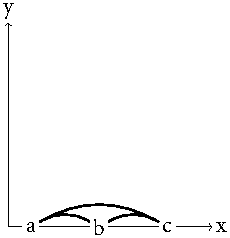
\includegraphics{figures/t_page_c3}
	\label{figure:page-c3}
	\caption[Page embedding of $C_3$]{A page embedding of $C_3$}
\end{figure}

\myref{figure:page-c3} depicts a page embedding for~$C_3$, the cycle on three~vertices.
By taking multiple page embeddings, we get a book embedding. 

\begin{definition}
\label{def:book-embed}
A \emph{book embedding} of graphs $G_1 = (V, E_1),\dotsc,\allowbreak G_k = (V, E_k)$ on the same set of vertices consists of page embeddings for each of the graphs that coincide in their vertex positions. 

In the setting of book embeddings the line $\SR \times \{0\}$
is also called the \emph{spine}. We only demand that edges in the same
graph~$G_i$ do not intersect. This can also be interpreted as giving each graph~$G_i$ its own upper half-plane, which we also call the \emph{page of~$G_i$}. Whenever we refer to a page in this thesis, we usually
mean the graph~$G_i$ on this page.
%The metaphor of an embedding into a book is then justified: The vertices are placed on the real line, the ``spine'' of the book, and the edges on their own copy of the upper half-plane, their ``page'' of the book. 
\end{definition}

The embeddability problem now asks whether such an embedding exists.
\newProb{\probBook}{A vertex set $V$ and edge sets $E_1,\dotsc, E_k \subseteq \binom{V}{2}$}
{Is there a book embedding of $(V, E_1),\dotsc, (V, E_k)$?}


In the literature \emph{book embedding} usually refers to the somewhat different problem \probBookNormal. Instead of directly embedding $k$~graphs
into $k$~pages, we first have to get $k$~graphs by arbitrarily partitioning the edges of a graph into 
$k$~parts and then embed these into $k$~pages. The problem
we call \emph{book embedding} is often called \emph{book embedding with fixed page assignment} in the literature. 
\newProb{\probBookNormal}{A vertex set $V$, an edge set~$E \in \binom{V}{2}$ and a number~$k\geq 1$}
{Is there a partition~$E = \bigcup_{i=1}^{k} E_i$ such that $(V, E_1), \dotsc, (V, E_k)$ is book embeddable?}
We depict this
assignment of the edges to the pages that has already been fixed either by using different colours or in the case of exactly two pages by one set of edges being drawn above and one below the spine.

\section{Related Work}
\label{section:related}

The \probBook problem is a graph drawing problem that is closely related to simultaneous planar drawings. Bläsius, Kobourov
and Rutter~\cite{GD2012} provide a good overview of those types of problems. 

In this section 
we first list some useful results about the usual book embedding problem \probBookNormal.
Then we present the literature about its variant \probBook.  
The fixed page problem \probBook had not been well-studied before the writing of this thesis. Thus, the list
of published results is quite small, even though it is exhaustive.

Furthermore, we introduce the concept of a \PQ-tree here, as first described by Booth and Lueker~\cite{Booth76}. Although \PQ-trees are not directly related to book embeddings,
we use them in many of the special cases in \myref{chapter:special}. Thus,
we also reference some results about \PQ-trees at the end of the section.

\begin{figure}[\placement]
    \centering
    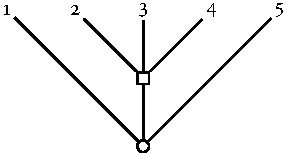
\includegraphics{figures/t_pq-tree}
    \caption[Simple \PQ-tree]{A simple \PQ-tree. \PT-nodes are drawn as a circle \tikz[scale=0.4,baseline={([yshift=+0.1em]current bounding box.south)}] \draw (0,0) circle (1em);, \Q-nodes as a box \tikz[scale=0.75,baseline={([yshift=+0.1em]current bounding box.south)}] \draw (-0.5em, -0.5em) -- ++(1em, 0) -- ++(0, 1em) -- ++ (-1em,0) -- cycle;.}
    \label{figure:pq}
\end{figure}

\begin{definition}\label{def:pq}
A \emph{\PQ-tree} $T$~on $M := \range{n}$ is a rooted, ordered
tree with leaves~$M$ and inner nodes either of type~$P$ 
or type~$Q$.

The tree represents a set of permutations $\pi(T) \subseteq \Sym(M)$ on its leaves as follows: The order of the children
of a \PT-node can be permuted in any way, while the order of the children of a \Q-node can only be reversed. The set~$\pi(T)$ then consists exactly of the permutations of the leaves~$M$ that we can get
by flipping the inner nodes in any of the specified valid ways.

The empty set of permutations on a set cannot normally be described by a \PQ-tree, so we define the	 special \emph{null tree} $\varepsilon$ representing~$\emptyset$.
Furthermore, let a \emph{\PT-tree} be a \PQ-tree containing only \PT-nodes as inner nodes and a \emph{\Q-tree} be a 
\PQ-tree only containing \Q-nodes as inner nodes.
\end{definition}

For example, the \PQ-tree in \myref{figure:pq} represents the permutations 12345, 14325, 52341, 54321, 15234,  15432,  51234,  51432, 23415, 43215, 23451 and 43251.

\paragraph{Book Embedding without Fixed Page Assignments}

We first enumerate some results for \probBookNormal. We do not use
these results, but they are still a helpful point of reference for classifying our
findings about the fixed page case \probBook.

There are a variety of results about small page numbers: The graphs
embeddable in a single page are just the outerplanar graphs and a graph
is embeddable into two pages if and only if it is \emph{sub-hamiltonian}, \ie a subgraph of a planar Hamiltonian
graph, as shown by Bernhart and Kainen~\cite{Bernhart79}. Widgerson~\cite{Widgerson82} proved
that checking a maximal planar graph for Hamiltonicity is \NP-complete, \ie \probBookNormal is already
\NP-complete if we restrict ourselves to two pages.

Thus, the book embedding problem for $k \ge 2$~pages is probably not efficiently solvable.
One viable research direction following this insight was to consider variations of the problem
or special graphs. Indeed, there are results for several graphs, including
but not limited to the following: A planar graph is embeddable into four pages~\cite{Yannakakis86},
a graph of treewidth~$k$ has book thickness at most~$k + 1$~\cite{Dujmovic07} and genus~$g$
graphs have book thickness~$\OO(\sqrt{g})$~\cite{Malitz88}. We do not explain these results further as we do not use them.

\paragraph{Book Embedding with Fixed Page Assignments}

In contrast, little is known about the variant \probBook with fixed page assignments. The only result we could find appears
in a recently published technical report by Hong and Nagamochi~\cite{two-page-09}. They show
that \probBook is decidable in linear time for two pages, unlike \probBookNormal. That is, the argument for the \NP-completeness of \probBookNormal
cannot be adopted for fixed page assignments. 

Furthermore, Angelini et.\,al.~\cite{angelini11} provide an interesting application for the
\probBook problem. They consider the important special case \SEFECON, whose complexity is unknown, of the simultaneous embedding problem \SEFE and reduce it to a 2-page \probBook problem where
the vertex order on the spine is additionally constrained by a \PT-tree.

\newProb{\SEFE}{Two graphs~$G_1$ and~$G_2$.}{Are there planar embeddings
of~$G_1$ and~$G_2$ that coincide on~$G_1 \cap G_2$?}
\newProb{\SEFECON\label{prob:sefecon}}{Two graphs~$G_1$ and~$G_2$ where~$G_1 \cap G_2$ is connected.}{Are there planar embeddings of~$G_1$ and~$G_2$ that coincide on~$G_1 \cap G_2$?}


\paragraph{PQ-trees}
The concept of a \PQ-tree was originally described by Booth and Lueker~\cite{Booth76} to solve
the consecutive ones problem: Given a 0-1-matrix, is there a permutation of its columns
such that the 1's in every row appear consecutively? Let~$T$ be a \PQ-tree and~$S$ some
subset of its leaves. Then they showed that there is an operation $\reduce(T, S)$, computable
in $\OO\bigl(|S|\bigr)$~time, that
yields a \PQ-tree representing exactly the permutations in~$\pi(T)$ where all leaves in~$S$ appear
consecutively. Thus, the consecutive ones problem can be solved by starting
with a \PQ-tree representing all permutations on the columns (a single \PT-node) and reducing on the columns containing~1's row by row. This reduction operation proves useful for solving the variations on
book embedding in \myref{chapter:special}. 

Booth~\cite{Booth75} additionally showed that we can intersect two \PQ-trees in linear
time, \ie from two \PQ-trees $T_1$ and $T_2$ on the same leaves we can construct a \PQ-tree representing~$\pi(T_1) \cap \pi(T_2)$ in linear time.

We also make use of the fact that there are linear time planarity algorithms that test a graph~$G$
for planarity and embed~$G$ vertex-by-vertex.
% such that at each have step and for each component of the
%already embedded graph we get a \PQ-tree that represents the possible orders of the half-embedded edges %in an
%extension of this partial embedding. 
The general scheme for these algorithms is summarised by Haeupler and Tarjan~\cite{Haeupler08}. 
Their scheme unifies and simplifies several similar linear-time planarity algorithms:
\begin{enumerate} 
\item The Lempel-Even-Cederbaum algorithm~\cite{Lempel67} that was refined
to run in linear time by Booth and Lueker~\cite{Booth76}
\item The Shih-Hsu algorithm~\cite{Shih93}
\item The Boyer-Myrvold algorithm~\cite{Boyer99}
\end{enumerate}

\section{Contribution and Outline}
\label{section:contrib}

From the literature analysis above we can see that there are a lot of open problems
for \probBook. For example: Is \probBook \NP-complete for a linear number
of pages? Does \probBook remain efficiently solvable for 3~pages? What happens when we constrain
the vertex orders by a \PQ-tree?

In this thesis we want to solve some of these open problems and provide points of reference for further
research. We first consider the time complexity of \probBook and then some special cases or restrictions thereof. More specifically, this work is structured as follows:

\begin{description}
\item[\myref{ch:preliminaries}] Firstly, we provide basic definitions and results
we need in the rest of the thesis. This is followed by rephrasing \probBook as a 
total ordering problem \probBookOrder. At the end of the chapter we begin to actually study book embeddings by identifying some of the freedoms we have in choosing total orders that solve an \probBookOrder instance. 
\item[\myref{chapter:complexity}] As alluded to above, in this chapter we show that the \probBook problem
is \NP-complete for an unbounded number of pages by reduction from the betweenness problem that is
also defined in this chapter. 
This result even applies if the edges on each page form a matching.

Since we still want to decide book embeddability for some graphs, we then show
how to solve \probBook in exponential time by expressing book embeddability using 3-\CNF-formulae. We also provide some optimisations for these formulae.
\item[\myref{chapter:special}] This chapter contains our main results. We discuss
and solve \probBook for several special cases and restrictions.

Firstly, we show that \probBook can be solved in linear time if each
page is a connected graph on all vertices. 

Then
we proceed with the opposite, the almost completely disconnected case, \ie we take disjoint perfect matchings as pages. We already
know that \probBook is \NP-complete for (general) matchings on the pages, at least if
we allow an unbounded number of pages. It is not clear whether perfect matchings make \probBook easier.

Still, we can give a necessary
criterion when the pages are perfect matchings, namely the union of all the pages has to be a bipartite graph. This criterion is not sufficient. Indeed, we then find both bipartite examples and counterexamples
for all numbers of pages, partly using computer assistance.

We continue with a variation on book embedding. Motivated by a result of Angelini et.\,al.~\cite{angelini11}, we consider book embeddings with the additional constraint that the
order of the vertices must be represented by a given \Q-tree. We show that this restricted case is
solvable in quadratic time.

The chapter closes with another variation on \probBook. We take multiple spines~(parallel lines)
in the plane and associate every vertex with a spine it has to be drawn on. 
Additionally, we impose the restriction that edges must be drawn between consecutive spines, above the
topmost spine or below the bottommost spine. Unlike the previous case, we do not solve this
variation. We just show that it is equivalent to
\probBook with 2~pages where the vertex order is constrained
by a special kind of \PT-tree. If we did not allow the edges to go
above the topmost or below the bottommost spine, this variation would be the same as the level planarity problem, which was first introduced by Tomii~et.~al.~\cite{Tomii77}. Jünger, Leipert and
Mutzel presented an algorithm that checks for level planarity in linear time~\cite{Junger99}.
\item[\myref{ch:conclusion}] The thesis is concluded by summarising the results
we obtained and discussing viable future research directions.
\end{description}

%This chapter should contain
%\begin{enumerate}
%  \item A short description of the thesis topic and its background.
%  \item An overview of related work in this field.
%  \item Contributions of the thesis.
%  \item Outline of the thesis.
%\end{enumerate}

%%% Local Variables: 
%%% mode: latex
%%% TeX-master: "thesis"
%%% End: 

	\chapter{Preliminaries}\label{ch:preliminaries}

\noindent As we noted in the introduction, this thesis is concerned with book embeddings with 
fixed page assignments, a variation on the
problem of embedding graphs in the plane without edge crossings.

Let us first review some basic results from graph theory before beginning to deal with book embeddings. 
For a more detailed treatment of the basics, consult any introductory
text on graph theory, \eg the book ``Graph Theory'' by Diestel~\cite{Diestel}.

\paragraph{Basic definitions}
Often, we want to draw graphs in the Euclidean plane, identified with $\SR^2$, without
edge crossings. Such a drawing is called a \emph{planar embedding}. If $G$ is
embeddable in the plane, we call it a \emph{planar graph}.

More formally, a \emph{planar embedding} of a graph $G = (V, E)$ consists of two
maps $m_V$ from $V$ to~$\SR^2$ and $m_E$ from $E$ to the set of continuous functions from $[0, 1]$ to~$\SR^2$ with the following properties:
\begin{enumerate}
\item The endpoints of the curve corresponding to an edge are the images of the curve's incident
vertices under $m_V$, \ie $m_E(e)(0) = m_V(a)$ and $m_E(e)(1) = m_V(b)$ for
all $e = \{a, b\} \in E$.
\item The curve $m_E(e)$ is injective (a \emph{Jordan curve}) and piecewise differentiable for all $e \in E$. 
%Such curves are called \emph{Jordan curves}.
\item Let $e_1, e_2 \in E$ be two different edges of $G$. Then $m_E(e_1)$ and $m_E(e_2)$ do not
intersect in their interiors $m_E(e_1)\bigl((0, 1)\bigr)$ and~$m_E(e_2)\bigl((0, 1)\bigr)$.
\item No image~$m_E(e)$ of an edge~$e \in E$ contains the image of any vertex apart from its endpoints.
\end{enumerate}

Removing the images~$m_E(e)$ of the edges~$e$ separates the plane into several connected
components. These components are called the~\emph{faces} of the embedding.

The graphs that can be drawn planarly such that all vertices
are on the boundary of a single face are the \emph{outerplanar graphs}, a subset of the set of planar graphs.
Let~$G$ be a graph and $\widetilde{G}$ be the extension that we get from~$G$ by adding a new vertex
adjacent to all vertices of~$G$. Clearly, $G$~is outerplanar
if and only if~$\widetilde{G}$ is planar.

Another basic fact is Euler's formula. It states that any planar embedding of
a graph with $v$~vertices and $e$~edges contains exactly $f = 2 + e - v$~faces. An edge
bounds at most two faces and a face's boundary contains at least three edges, \ie $3f \le 2e$ (exception: a single edge).  With
Euler's formula we can, thus, bound the number of edges of a planar graph
by $6 + 3e - 3v = 3f \le 2e \iff e \le 3v - 6$. Applying this bound to the extended planar graph
belonging to an outerplanar graph yields $e + v \le 3(v + 1) - 6 \iff e \le 2v - 3$ since the
extended graph has $v$~additional edges and $1$~additional vertex. Thus, an $n$-vertex
outerplanar graph has at most $2n - 3$ edges. Equality occurs for $C_n$, the cycle on $n$~vertices, with
additional edges from one vertex to all of the $n-3$~other vertices it is not adjacent to (a triangulation of~$C_n$).

\paragraph{Book embedding}



With these basic definitions out of the way, we can return to the page embeddings of \myref{def:page-embed}. The problem of deciding whether a page embedding exists is not very interesting.
The embeddable graphs are exactly the outerplanar graphs~\cite{Bernhart79}.
Thus, we get the necessary condition \nopagebreak$|E| \leq 2|V| - 3$
for page embeddability.

The problem becomes significantly harder when we have $k$~pages as for the book embeddability problem \probBook. For the case~$k=1$ we just saw that checking for book embeddability is the same as checking for outerplanarity, which can be done by adding one vertex
adjacent to all other vertices and testing planarity. Hong and Nagamochi~\cite{two-page-09} 
showed that \probBook is solvable in linear time for~$k=2$. In particular, it remains efficiently solvable. The general problem for arbitrary~$k$ had not been considered before this thesis.

We already know that $|E_i| \leq  2|V| - 3$ for all~$i \in \range{k}$ is necessary for book
embeddability.
That is, the number of edges~$|E_i|$ is linear in~$|V|$ for all~$i \in \{1,\dotsc, k\}$. Furthermore, in all complexity considerations we assume the
number of pages to be constant. All in all, the size of a book embedding instance is in~$\OO\bigl(|V|\bigr)$.

We now have some idea of the problem we want to consider. 
To familiarise ourselves even more with book embeddings, firstly, this chapter reduces \probBook to a total ordering problem \probBookOrder that we can work with more easily~(\myref{section:total-ordering}).
Secondly, we show what freedoms we have in choosing total orders that solve a \probBookOrder instance~(\myref{section:symmetry}). This allows us to gain insight into the choices the problem leaves us, which proves useful for showing \NP-completeness in~\myref{section:np-complete}.

\section{Book Embedding as Total Ordering Problem}
\label{section:total-ordering}

At first sight the book embedding problem looks like a geometric problem, where
the actual page drawings are important.
Since there are lots of different embeddings that differ just slightly in how they map the edges to curves, this would make the problem quite unwieldy.

In this section we show that the first impression deceives. Only the order of the vertices on the spine is significant for testing embeddability. Thus, we can turn the book embedding problem into a total ordering problem. In this thesis we always mean strict total orders when we speak about total orders.

We first show that a single page embedding corresponds to an ordering problem.
\begin{definition}\label{def:book-constraint}
Let~$(V, E)$ be a graph and~$<$ a total order on~$V$.
We call the condition that the suborder $a < c < b < d$ does not occur for any $\{a, b\}, \{c, d\} \in E$ the
\emph{book constraint for~$E$}. If~$<$ fulfils the book constraint for~$E$ we say that it is a \emph{valid book order for~$E$}. 
\end{definition}
\begin{lemma}
\label{lemma:constraints}
There is a page embedding for $G = (V, E)$ if and only if there is a valid book order~$<$ 
for~$E$.
\end{lemma}
\begin{myproof}
\begin{itemize}
\item[]
\item[``$\Rightarrow$'']
Let there be a page embedding of $G$ with vertex map $m_V$ and
edge map $m_E$. We use $m_V$ to define the
ordering via $u < v :\Leftrightarrow m_V(u) < m_V(v)$ for all $u, v \in V$.

If $a < c < b < d$ occurs for some $\{a, b\}, \{c, d\} \in E$, then the Jordan curves
$m_E\bigl(\{a, b\}\bigr)$---from $a$ to $b$---and $m_E\bigl(\{c, d\}\bigr)$---from $c$
to $d$---have to intersect, as illustrated in \myref{figure:total}, since they lie in the upper half-plane. 

More formally, we can add the spine to any page embedding by drawing straight lines between 
consecutive vertices on the spine and a curve in the upper half-plane from the leftmost vertex on the spine to the
rightmost vertex on the spine such that planarity is preserved.
This construction results in an outerplanar embedding since  all vertices still lie in the component the \emph{lower half-plane $\bigl\{(x, y) \in \SR^2\colon y < 0\bigr\}$} belongs to. By doing this
construction for the given page embedding of the edges $\{a, b\}$ and  $\{c, d\}$ we get
an outerplanar embedding of the complete graph on four vertices~$K_4$, as illustrated in \myref{figure:total}. This is a impossible since~$K_4$ is not outerplanar. Thus, the
book constraint must be fulfilled.

%More formally, let~$C$ be the concatenation of $m_E(\{a, b\})$ with the segment of the real line from $b$ to~$a$. Then~$C$ is a Jordan loop, a continuous loop without self-intersections. By Jordan's curve theorem, $\SR^2 \setminus C$ has two connected components that we call the inside and the outside and any curve from a point in one component
%to a point in the other component intersects~$C$. Now consider~$m_E(\{c, d\})$. The point~$c$ is on~$C$
%and the point~$d$ is in the outside. Since the interior of~$m_E(\{c, d\})$ lies in the upper half-plane, it has to contain a point~$P$ in the inside near to~$c$. Thus, the segment of the curve $m_E(\{c, d\})$ from $P$ to~$d$ intersects~$C$ by the Jordan curve theorem. This intersection has to occur in the curve~$m_E(\{a, b\})$ as this segment has no point in common with the real line apart from~$d$.

\item[``$\Leftarrow$'']
Let $<$ be valid book order for~$E$ and $i(v)$ denote the index of $v$ in $<$ for
all $v \in V$, \ie $i(v) = j$ if and only if $v$ is the $j$-th smallest element in~$V$
according to~$<$.
 
Then we define the page embedding as follows. The vertex map $m_V$ maps a vertex~$v$ 
to the real number~$i(v)$ and the edge map $m_E$ maps an edge~$\{a, b\}$ to the semi-circle
in the upper half-plane that has
the line segment $m_V(a)m_V(b)$ as diameter.

Now let $e_1 := \{a, b\}, e_2 := \{c, d\}$ be different edges of $G$.
If two of $a$, $b$, $c$ and~$d$ are the same, the semi-circles
$m_E(e_1)$ and~$m_E(e_2)$ of different size share an endpoint, \ie they do not intersect in their
interior and we are done. 

So assume $a$, $b$, $c$ and~$d$ are pairwise distinct
as well as \[ \text{$a < b$, $c < d$ and $a < c$} \tag{1}\] without
loss of generality.

The curve $m_E(e_1)$ is a semi-circle with centre $\bigl(i(a) + i(b)\bigr)/2$ and radius $\bigl(i(b) - i(a)\bigr)/2$. Similarly, the curve $m_E(e_2)$ is a semi-circle with centre $\bigl(i(c) + i(d)\bigr)/2$ and radius $\bigl(i(d) - i(c)\bigr)/2$.
Since we assumed~(1), these semi-circles intersect in their interior if and only if $i(c) < i(b) < i(d)$.
With $a < c$ this would mean $a < c < b < d$ in contradiction to the assumption.

Therefore, no two semi-circles corresponding to different edges intersect in their interior,
\ie $(m_V, m_E)$ is a valid page embedding.\qedhere
\end{itemize}
\end{myproof}

\begin{figure}[\placement]\centering
    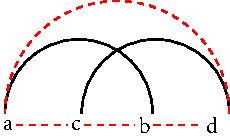
\includegraphics{figures/t_total_order}
    \caption[Book embedding constraints]{If $a < c < b < d$ occurs for two edges $\{a, b\}$ and $\{c,d\}$,
there is no page embedding with the order~$<$. Especially not a canonical one using semi-circles. The
red (dashed) edges result from adding the spine to the page embedding.}
    \label{figure:total}
\end{figure}

\noindent Since the pages in a book embedding problem are independent of each
other, we can use this lemma to rephrase the book embedding problem
as a total ordering problem.
\newProb{\probBookOrder}{A finite set $V := \range{n}$ and sets
$E_1,\dotsc, E_k \subseteq \binom{M}{2}$.}
{Is there a valid book order $<$ for all~$E_i$ where $i \in \range{k}$?}
\begin{theorem}
\label{lemma:all-book-constraints}
\probBook and \probBookOrder are equivalent.
\end{theorem}
\begin{myproof}
Follows by applying \myref{lemma:constraints} to each page.\qedhere
\end{myproof}

From this point onward, we use both representations of the book embedding problem
interchangeably. Whenever we refer to \probBook we also mean \probBookOrder and vice versa.
Note that the book constraints for two edges $\{a, b\}$ and $\{c, d\}$ are trivially fulfilled if
the edges have a common vertex. Therefore, we always assume that two edges are independent whenever
we check book constraints in the remainder of the thesis.

\section{Equivalent Orders}\label{section:symmetry}

We significantly reduced the number of basically equivalent ways to solve a book
embedding instance by restating the drawing problem \probBook as an ordering problem \probBookOrder. Still, several choices remain.
We determine some of them in this section, namely that the mirror image and any cyclic shift of a total order solving a \probBook instance still solve the instance. 

Notably, this knowledge proves useful for reducing other problems to book embedding in 
\myref{chapter:complexity} where we discuss the time complexity of \probBook.

By considering all mirror images and cyclic shifts of a total order to be the same
we turn the total order into what we call a \emph{symmetric order}.

\begin{figure}[\placement]\centering
    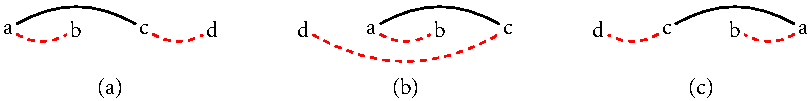
\includegraphics[width=\textwidth]{figures/t_symmetry}
    \caption[Equivalent orders]{A valid book embedding (a) with cyclic shift to the right by one element~(b)
and mirror image~(c).}
    \label{figure:symmetry}
\end{figure}

%\begin{definition}
Let~$M$ be an $n$-element set and~$O_M$ be the set of total orders (permutations) on~$M$.

For a permutation $\pi = (a_1, a_2, \dotsc, a_n) \in O_M$ we say that~$(a_n, a_{n-1}, \dotsc, a_1) \in O_M$ is the \emph{mirror image of~$\pi$} and~$(a_{n-k+1}, a_{n-k+2}, \dotsc, a_n, a_1, \dotsc, a_{n-k}) \in O_M$ is the \emph{cyclic shift of~$\pi$ by~$k$} for~$k \in \{0, \dotsc, n-1\}$. Both of these elementary operations are illustrated in \myref{figure:symmetry}.

We now define a relation~$\sim$ on~$O_M$. For all $a, b \in O_M$ we have
$a\sim b$ if and only if we can get~$b$ from~$a$ by a series of cyclic shifts
and mirror images. Clearly, the relation~$\sim$ is an equivalence relation.

Let~$\widetilde{O}_M$ be the set of equivalence classes of~$O_M$ with respect to~$\sim$. An
element~$o \in \widetilde{O}_M$ is then called a \emph{symmetric order on~$M$}. We write~$[\pi] := \{\tau \in O_M: \pi \sim \tau\} \in\widetilde{O}_M$ to refer to the symmetric order corresponding to a permutation~$\pi \in O_M$.
%A ternary relation~$[\cdot, \cdot, \cdot]$ on a set~$M$ is called a \emph{cyclic order} if the
%following constraints hold for all~$a, b, c, d \in M$:
%\begin{enumerate}
%\item If $[a, b, c]$, then~$[b, c, a]$. (\emph{cyclic})
%\item If $[a, b, c]$, then not $[c, b, a]$. (\emph{asymmetric}).
%\item If $[a, b, c]$ and $[a, c, d]$, then $[a, b, d]$. (\emph{transitive})
%\item If $a$, $b$ and $c$ are pairwise distinct, then either $[a, b, c]$ or
%$[c, b, a]$. (\emph{total})
%\end{enumerate}
%\end{definition}

Let~$<$ be a total order (permutation) on a finite set~$M$. We can order the elements
of~$M$ on a circle by starting at one point of the circle, going either clockwise
or counter-clockwise without making a full turn and writing the elements of~$M$ on distinct points in the order~$<$. 

Conversely, if we have an arrangement of a finite number of elements on distinct points of a circle, it is ambiguous which total order we got this arrangement from. We can cut the circle open between any two elements and get a total
order by going either clockwise or counter-clockwise. Clearly, the notion of a symmetric order is defined
exactly in such a manner that the orders we get from~$<$ (written on a circle) by cutting the circle open are the orders~$[<]$.

That is, a symmetric order can alternatively be interpreted as a way of ordering elements on a circle.
If we only consider cyclic shifts in the definition of~$\sim$, we get \emph{cyclic orders} which are
considered more often in the literature.
%It is unusual that we do not distinguish between the two directions (clockwise or counter-clockwise) of %the order, but we stick with this definition in this thesis.
%The natural interpretation of $[a, b, c]$ is: after~$a$, one
%reaches~$b$ before~$c$ on the cycle. Any linear order on~$M$ can be turned into a cyclic
%order by writing the elements of~$M$ from the smallest to the
%largest on a cycle. Similarly, we can get a linear order from a cyclic order
%by starting at any element and walking around the cycle in one direction.
%When turning a linear order~$<$ into a cyclic order and then transforming it into
%a linear order again, a different linear order may result. We call these orders \emph{cyclic rotations}
%of the original order~$<$. All of them can be constructed by a series of reflections and
%shifts to the right. Both of these elementary operations are illustrated in \myref{figure:symmetry}. We now show that any cyclic rotation of a valid book order remains valid.

We now show that cyclic shifts and mirror images preserve the validity of an order.

\begin{theorem}
\label{lemma:symmetry}
Let $(V, E_1),\dotsc, (V, E_k)$ be a book embedding instance with valid book order~$<\,\in O_V$.
Then any order $<_c\,\in [<]$ is valid.
\end{theorem}
\begin{myproof}
We show that the cyclic shift by one~$<_1$ of~$<$ and
the mirror image~$<_2$ of~$<$ are still valid orders. Then any order~$<_c\,\in [<]$ must also be valid.

To do so we show that a page~$(V, E_i)$ cannot have the forbidden substructure of \myref{lemma:constraints} in either order $<_1$ or~$<_2$.

If $a <_2 c <_2 < b <_2 d$ occurs for some~$\{a, b\}, \{c, d\} \in E_i$, we have $d < b < c < a \in E_i$ as $<_2$ is the reverse of~$<$, which
contradicts the validity of~$<$. Thus,~$<_2$ must be valid.

Similarly, assume the forbidden substructure $a <_1 c <_1 b <_1 d$ occurs for some~$\{a, b\}, \{c, d\} \in E_i$. If~$a$ is not the smallest element of~$V$ with respect to~$<_1$, we get~$a < c < b < d$ by construction of~$<_1$, a
contradiction to the validity of~$<$. Otherwise,
we get $c < b < d < a$, which again contradicts
the validity of~$<$. Thus,~$<_1$ is valid.
\end{myproof} 
 
%By applying an appropriate continuous
%deformation to it,  every page drawing is mapped to a planar drawing where all the
%vertices are on the unit circle and all edges lie inside of it.

%Reversely, there is a continuous deformation mapping the unit sphere
%to the upper half-plane and an arbitrary vertex on the cycle
%to the left-most vertex on the real line as well as traversing the cycle in an arbitrary
%direction. That is, we get a book embedding
%for all cyclic rotations of~$<$.
%%If we fix a book drawing with order $>$ and consider $\SR^2$
%%as the complex plane $\SC$, this is fairly clear:
%%Just apply the Mobius transformation $f$ which maps $\SR$ to the unit circle,
%%then the appropriate rotation around the origin and finally $f^{-1}$ to the drawing. This
%%yields a book drawing with the cyclic rotation as vertex order. Note that
%%the Mobius transformation~$f$ maps the half-planes bounded by $\SR$ to the half-planes
%%bounded by the unit circle, \ie the edges still lie in one of the half-planes bordered
%%by~$\SR$.
%\end{myproof}
%
%Since the validity of the order remains invariant under cyclic rotations, 
%the ordering problem for book embeddings is sometimes defined on cyclic
%orders. This is not significant, since a cyclic order can always be cut open at any vertex to 
%return to our setting of total orders. For this reason, we use cyclic orders and linear orders interchangeably in this thesis.
%%% Local Variables: 
%%% mode: latex
%%% TeX-master: "thesis"
%%% End: 

	\chapter{Algorithmic Complexity}
\label{chapter:complexity}

The book embedding problem  without fixed page assignments  \probBookNormal is \NP-complete. For two pages
Bernhart~\cite{Bernhart79} showed that the problem is the same
as determining whether the graph is \emph{sub-hamiltonian}, \ie a subgraph of a planar
graph with a Hamiltonian cycle. This implies that \probBookNormal is \NP-complete by a result of Widgerson's~\cite{Widgerson82},
which states that the Hamiltonian circuit problem for maximal planar graphs is \NP-complete.

Since the two page case with fixed partitions is solvable in linear time~\cite{two-page-09},
we see that fixing the partitions significantly changes the book embedding problem. Is \probBook even
\NP-complete? We answer this question in the affirmative in the first
half of this chapter (\myref{section:np-complete}),
but, unfortunately, only for an unbounded number of pages. 

Thus, we know that \probBook is probably not efficiently solvable. In spite of that, we
want to test some specific instances in \myref{section:matchings}.
For this reason, in the second half of
this chapter~(\myref{section:sat}) we show how \probBook can be solved in super-polynomial time  by reducing it to \probThreeSat with some optimisations.
We chose the \probThreeSat problem since there are solvers for it that work well
on instances occurring in practice, even though \probThreeSat is \NP-complete.

\section{\textsc{Book-Embedding} is \NP-Complete}
\label{section:np-complete}

In this section we
construct a polynomial-time reduction from the \NP-complete problem \probBetween, defined below,
to \probBook, \ie we show that \probBook is \NP-complete. Therefore,
we cannot expect there to be an efficient algorithm for solving the general
book embedding problem.

Checking the book constraints for a pair of edges takes $\OO(1)$~time
and there are $\OO\bigl(\sum_{i} |E_i|^2\bigr)$ pairs to check.
Thus, checking the validity of a guessed book order takes polynomial
time and the book embedding problem must, therefore, be in~\NP.

We now give a polynomial time reduction from the problem \probBetween, which was shown to be \NP-complete by Opatrny~\cite{opatrny:79}, to \probBook and, thereby, show that \probBook itself is \NP-complete.

\newProb{\probBetween}{A finite set $M := \range{n}$ and a set of ordered triples $C \subseteq M^3$.}
{Is there a total ordering $<$ of $M$ such that either $a < b < c$ or $a > b > c$ occurs for all $(a, b, c) \in C$?}

The idea of the reduction is to map each triple to edges on two new pages that form a $C_4$, a cycle on 4~vertices. By
the following lemma, these two pages exactly represent the betweenness constraint.

\begin{figure}[\placement]\centering
    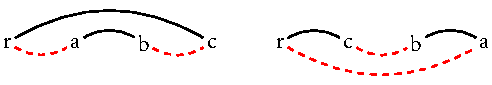
\includegraphics{figures/t_np_c4}
    \caption[Drawings of $C_4$]{The two drawings of a $C_4$ starting at $r$}
    \label{figure:np-c4}
\end{figure}

\begin{lemma}
\label{lemma:np-c4}
Let $V := \{r, a, b, c\}$, $E_1 := \bigl\{\{r, a\},\{b, c\}\bigr\}$ and $E_2 := \bigl\{\{a, b\}, \{r, c\}\bigr\}$. Then
$r < a < b < c$ and $r < c < b < a$, depicted in \myref{figure:np-c4}, are the only valid book embeddings of $E_1$ and $E_2$ with 
$r$ as first vertex.
\end{lemma}
\begin{myproof}
Let $<$ be a valid book order on $V$.
By \myref{lemma:constraints} the two pages yield the constraints $r < b < a \Leftrightarrow r < c < a$
and $r < a < c \Leftrightarrow r < b < c$. Since $r$ is the smallest element of $<$, this
is the same as $b < a \Leftrightarrow c < a \Leftrightarrow c < b$, \ie only the two cases $r < a < b < c$ and
$r < c < b < a$ remain.
\end{myproof}

Now let's do the formal reduction.

\begin{theorem}
\label{lemma:np-hard}
There is a polynomial time reduction from \probBetween to \probBook. Thus,
\probBook is \NP-complete.
\end{theorem}
\begin{myproof}
Let $I := (M, C)$ be a betweenness instance. 

Construct a book embedding instance $f(I) := \bigl(V, \bigcup_{t \in C} \left(E_{t,1} \cup E_{t,2}\right)\bigr)$ as follows.
Take $V := M\,\cup\,\{r\}$ as vertex set where $r \not\in M$ is a new symbol. For each triple $\tau~=~(a, b, c) \in C$ introduce
two new pages $E_{\tau, 1} := \bigl\{\{r, a\}, \{b, c\}\bigr\}$ and $E_{\tau, 2} := \bigl\{\{a, b\},\{r, d\}\bigr\}$. The instance $f(I)$ can obviously 
be computed in polynomial time.

Now show that $I$ is a positive instance if and only $f(I)$ is one.\nopagebreak
\begin{itemize}
\item[``$\Rightarrow$''] Let $I$ be a positive instance of \probBetween with valid total order $<$. Extend~$<$ to $V$ via
$r < k$ for all $k \in M$. For each triple $(a, b, c) \in C$ we have $r < a < b < c$ or $r < c < b < a$, \ie $<$ yields
a valid embedding of the pages by \myref{lemma:np-c4}. Thus, $<$ is a correct solution of $f(I)$.

\item[``$\Leftarrow$''] Let $f(I)$ be a positive instance of \probBook with valid total order~$<$. By \myref{lemma:symmetry} we
can assume  without loss
of generality that~$<$ is rotated such that $r$ is its smallest element. Then we have the situation of \myref{lemma:np-c4} for each triple $\tau = (a, b, c) \in C$ with
the pages~$E_{\tau,1}$ and $E_{\tau,2}$, \ie $a < b < c$ or $c < b < a$. Therefore, the order~$<$ restricted to $M$ is indeed a valid solution of $I$.\qedhere
\end{itemize}
\end{myproof}

We conclude that \probBook is \NP-complete. The reduction of
\myref{lemma:np-hard} gives us even more. The pages it creates are
matchings, \ie even the special case \probNotMatching of book embedding where the
edges on each page form a matching remains \NP-complete.

\newProb{\probNotMatching}{A vertex set $V$ and matchings $E_1, \dotsc, E_k \subseteq \binom{V}{2}$}%
{Is there a book embedding of $(V, E_1), \dotsc, (V, E_k)$?}

We do not know how complex the problem is when the edges on the pages form perfect matchings. This
special case is considered in more detail in \myref{section:matchings}.
%\begin{theorem}
%\label{theorem:np-complete}
%\probBook is \NP-complete.
%\end{theorem}
%\begin{myproof}
%Follows immediately from \myref{lemma:np-hard}.
%\end{myproof}
\section{Reduction to \probThreeSat}
\label{section:sat}

In the previous section we saw that~\probBook is \NP-complete.
This implies that we cannot expect to solve a general book embedding instance in polynomial time. 
But we still want to be able to check some instances, \eg to find counterexamples in special
cases as in \myref{section:matchings}. We, therefore, make it the goal
of this section to give a super-polynomial time algorithm for deciding book embeddability.

In order to achieve this, we express \probBook as a satisfiability problem of a Boolean formula.
The translation immediately yields a Boolean formula in 3-\CNF. That is,
the formula is a conjunction of disjunctions of literals (positive or negative variables) and each
disjunction contains at most~3 literals. The problem of deciding satisfiability for
these Boolean formulae is called~\probThreeSat and has been studied extensively.

\newProb{\probThreeSat}{A 3-\CNF Boolean formula \bool{f}.}{Is~\bool{f} satisfiable?}

Although \probThreeSat was the first problem to be proven \NP-complete~\cite{Cook71}, there
are \SAT-solvers that handle many instances occurring in practice in reasonable times. One that
has scored well in several contests is~\mytt{minisat}~\cite{minisat03}. We use it to 
check the resulting formulae for some instances in \myref{section:matchings}.

Now we derive the translation of the total order formulation of~\probBook from \myref{lemma:constraints}
into a Boolean formula. Let $\bigl((V, E_1),\dotsc, (V, E_k)\bigr)$ be the book embedding 
instance and label the vertices $V = \range{n}$ without loss of generality. 

We have to express the total order~$<$ as a set of Boolean variables. 
It is natural to introduce a variable
\bool{v(i, j)} for the statement $i < j$ for all $i, j \in V$. 

Then we have to build a 3-\CNF formula that rephrases the stipulation that~$<$ is a
strict total order and that the book constraints are fulfilled. We can achieve this by forming the conjunction of the following formulae.

\paragraph{Strict total order}

That~$<$ is a strict total order means, by definition, that it is asymmetric, irreflexive, transitive
and total:

\begin{description}
\item[irreflexive] For each vertex~$i \in V$ the formula~$i < i$ is false. 
We get~$\lnot v(i, i)$. (n~clauses)
\item[asymmetric and total] For each unordered pair of distinct vertices~$i, j \in V$ exactly one
of~$i < j$ or~$j < i$ is true. We get~$v(i,j) \xor v(j,i) \equiv \bigl(v(i,j) \lor v(j,i)\bigr) \land \bigl(\lnot v(i,j) \lor \lnot v(j,i)\bigr)$. (two~clauses for each of the $\binom{n}{2}$~unordered pairs)
\item[transitive] For each triple~$i, j, k \in V$ of vertices, if~$i < j$ and $j < k$ are
true, then also~$i < k$. We get~$\bigl(v(i, j) \land v(j, k)\bigr) \Rightarrow v(i, k) \equiv \lnot v(i, j)
\lor \lnot v(j, k) \lor v(i, k)$. (one clause for each of the $n(n-1)(n-2)$~ordered triples of
distinct vertices)
\end{description}

\paragraph{Book constraints}

For each unordered pair of different edges~$e_1 := \{a, b\}, e_2 := \{c, d\} \in E_i$, we have to take the book 
constraint from \myref{def:book-constraint} into account. The constraint says exactly that~$c$ is between~$a$
and~$b$ if and only if~$d$ is between~$a$ and~$b$ as well as that~$a$ is between~$c$ and~$d$
if and only if~$b$ is between~$c$ and~$d$. 

% We rephrase it as follows: If one
%vertex of one of the two edges lies between the vertices of the other, then the other 
%vertex of the first edge also lies between the vertices of the second. Furthermore, we have to
%consider all possible orders of $a$~and~$b$ respectively $c$~and~$d$.

That is, if we choose one of the edges $e_1$ or~$e_2$ as edge~$e_O := \{w, x\}$ and the other as
edge~$e_I := \{y, z\}$, we get the following equivalence:
\[
%\bigwedge_{\substack{e_O, e_I \in \{e_1, e_2\}\\e_I \neq e_O, e_I =: \{y, z\}}} \bigwedge_{\substack{w, %x \in e_O\\w \neq x}} \Bigl(v(w, y) \land v(y, x) \Leftrightarrow v(w, z) \land v(z, x)\Bigr) 
\bigl(v(w, y) \land v(y, x) \Leftrightarrow v(w, z) \land v(z, x)\bigr) \tag{1}
\]
Exchanging the vertices $y$ and~$z$ does not change the resulting clauses, while
exchanging the vertices $w$ and~$x$ does. Thus, there are two choices to make. Firstly,
which of $e_1$ and~$e_2$ gets the name~$e_O$ and which gets the
name~$e_I$ (two possibilities). Secondly, which incident vertex of the edge~$e_O$ gets the
name~$w$ and which gets the name~$x$ (two possibilities).

Since the formula~(1) is equivalent to the \CNF-formula $\bigl(\lnot v(w, y) \lor \lnot v(y, x) \lor v(w, z)\bigr) \land\allowbreak\bigl(\lnot v(w, y) \lor \lnot v(y, x) \lor v(z, x)\bigr) \land \bigl(\lnot v(w, z) \lor \lnot v(z, x) \lor v(w, y)\bigr) \land \bigl(\lnot v(w, z) \lor \lnot v(z, x) \lor v(y, x)\bigr)$, we get $\text{2}\cdot \text{2} \cdot \text{4} = \text{16}$ clauses for each of
the $\sum_{i=1}^{k} \binom{|E_i|}{2}$ unordered pairs of edges.

We actually do not need the clauses for both choices of~$e_O$. Once the \SAT-formulae for one choice have been added, the constraints for the other choice immediately follow.

We now show this observation. Let $e_1 := \{a, b\}, e_2 := \{c, d\}$ be edges and
assume we have the \SAT-formulae of type~(1) with $e_O = e_1$ as well as the \SAT-formulae for the asymmetry and totality. 
We now show $v(c, a) \land v(a, d) \Rightarrow v(c, b) \land v(b, d)$. The other
instances of~(1) with~$e_O = e_2$ can be proven analogously. 

Assume that $v(c, a) \land v(a, d)$ is true.
If~$v(d, b)$ is true, we can infer $v(a, c)$ by $v(a, d) \land v(d, b) \Leftrightarrow
v(a, c) \land v(c, b)$ (the formula~(1) with $e_O = \{a, b\}$, $w = a$ and $x = b$) which contradicts $v(c, a)$ because of the asymmetry constraint. 
That is, $v(b, d)$~must be true by the asymmetry and totality.
In the
same manner we can show~$v(c, b)$. Thus, the assumption implies $v(c, b) \land v(b, d)$,
as desired.

This small optimisation saves half of the clauses,
\ie we only need eight~clauses for each pair of edges.

\paragraph{Fixed minimum}

From \myref{lemma:symmetry} we know that cyclic shifts preserve the validity of~$<$.
To help the \SAT-solver, we can, therefore, assume that~$1$ is the
smallest vertex and add the clauses~$v(1, j)$ for all $j \in V$ with $j \neq 1$. They
comprise another~$n-1$ clauses.

\begin{table}[tb]
\centering

\resizebox{\textwidth}{!}{
\begin{tabular}{lll}

\textbf{Axiom} & \textbf{3-\CNF formula} & \textbf{Number of clauses}\\
\toprule
Irreflexive          & $\lnot v(i, i)$ & $n$ \\
\midrule
Asymmetric and total & $\bigl(v(i,j) \lor v(j,i)\bigr) \land \bigl(\lnot v(i,j) \lor \lnot v(j,i)\bigr)$ & $2\binom{n}{2}$\\
                     & for all distinct unordered pairs $i, j \in V$ \\
\midrule
Transitive           & $\lnot v(i, j) \lor \lnot v(j, k) \lor v(i, k)$ & $n(n-1)(n-2)$\\ 
                     & for all ordered triples $i, j, k \in V$ where\\
                     & $i$, $j$~and $k$ are pairwise distinct\\
\midrule
Book embedding       & $\bigl(\lnot v(w, y) \lor \lnot v(y, x) \lor v(w, z)\bigr)$ & $16\cdot\sum_{i=1}^{k} \binom{|E_i|}{2}$\\
                     & $\land \bigl(\lnot v(w, y) \lor \lnot v(y, x) \lor v(z, x)\bigr)$ \\
                     & $\land \bigl(\lnot v(w, z) \lor \lnot v(z, x) \lor v(w, y)\bigr)$ \\
                     & $\land \bigl(\lnot v(w, z) \lor \lnot v(z, x) \lor v(y, x)\bigr)$ \\
                     & for all distinct $e_O = \{w, x\}$, \\
                     & $e_I = \{y, z\} \in E_i$ and all $i \in \range{k}$ \\
                     & where it matters which edge is\\
                     & assigned to $e_O$ and which to $e_I$\\
\midrule
Book embedding       & $\bigl(\lnot v(w, y) \lor \lnot v(y, x) \lor v(w, z)\bigr)$ & $8\cdot\sum_{i=1}^{k} \binom{|E_i|}{2}$\\
(optimised)          & $\land \bigl(\lnot v(w, y) \lor \lnot v(y, x) \lor v(z, x)\bigr)$ \\
                     & $\land \bigl(\lnot v(w, z) \lor \lnot v(z, x) \lor v(w, y)\bigr)$ \\
                     & $\land \bigl(\lnot v(w, z) \lor \lnot v(z, x) \lor v(y, x)\bigr)$ \\
                     & for all distinct $e_O = \{w, x\}$,\\
                     & $e_I = \{y, z\} \in E_i$ and all $i \in \range{k}$\\
                     & where it does not matter which edge is\\
                     & assigned to $e_O$ and which to $e_I$\\
\midrule
Fixed minimum         & $v(1, j)$ for all $j \in \bigl(V \setminus \{1\}\bigr)$ & $n - 1$\\
\bottomrule
\end{tabular}}

\caption[\CNF translation of \probBook]{The 3-\CNF formulae corresponding to \probBook}
\label{table:sat}
\end{table}

The clauses we get are summarised in \myref{table:sat}. They
provide us with a polynomial-time reduction from~$\probBook$ to~$\probThreeSat$.
The number of edges $|E_i|$ is linear in $|V|$ for all~$i \in \range{k}$ since~$(V, E_i)$ is an outerplanar graph.
Thus, we get~$\OO\bigl(|V|^3 + k|V|^2\bigr)$ clauses.

\begin{theorem}
Let~$I := (V, E_1, \dotsc, E_k)$ be a~$\probBook$ instance. There is a $\OO\bigl(|V|^3 + k|V|^2\bigr)$~time reduction
to an equivalent $\probThreeSat$ instance with~$\OO\bigl(|V|^3 + k|V|^2\bigr)$ clauses.
%$\probBook \leq_P \probThreeSat$
\end{theorem}
%\begin{myproof}
%The translated constraints in \myref{table:sat} which we can write down
%in polynomial time directly express the book embedding problem as 3-\prob{cnf} formula.
%\end{myproof}

%%% Local Variables: 
%%% mode: latex
%%% TeX-master: "thesis"
%%% End: 

	\chapter{Special Cases and Restrictions}
\label{chapter:special}

Having proven that \probBook is a hard problem in the previous section,
we now turn to some special instances or variations on \probBook and
either show how they can be solved efficiently or why they remain hard.
This section is the main contribution of this thesis.

One topic we are interested in is how embeddability depends
on the connectivity of the pages. Thus, we deal with both extreme
cases with regards to connectivity in the first two sections: The pages
can either all be connected~(\myref{section:connected}), or ``maximally
disconnected'' without isolated vertices~(\myref{section:matchings}), \ie consisting of perfect disjoint matchings.

We show that the connected case---quite surprisingly---admits a solution
in linear time.
For each page we get a \PQ-tree (see \myref{def:pq}) that stands for the
possible orders of the vertices in a page embedding of this single page.
The solution intersects these sets of orders to decide embeddability. 

In contrast, we are unable to provide an efficient algorithm if the edges of each
page form perfect disjoint matchings. We only manage to prove for this
case that an embeddable graph must be bipartite. Furthermore, we derive---by hand and using a computer---positive bipartite instances and the smallest bipartite counterexamples for all numbers of pages with the
exception of three pages. For three pages we are able to get a smallest counterexample
when two of the matchings form a cycle.

Another interesting restriction we make in \myref{section:trees} is to allow the order of the 
vertices on the spine to only come from the
permutations represented by a fixed \PQ-tree. We present a quadratic time algorithm
for solving the book embedding problem with this restriction if we only allow \Q-trees.
Angelini et.\,al.~\cite{angelini11} showed that a similar restriction is important by reducing \SEFECON~(see page~\pageref{prob:sefecon}) to a book embedding problem
with 2~pages constrained by a \PT-tree.

Finally, in \myref{section:multi_spine} we give a related 
variation on the book embedding problem. We now allow multiple spines~(parallel lines) in the plane
and associate every vertex with a spine the vertex has to be drawn on. 
Additionally, we demand that edges are drawn between consecutive spines, above the
topmost spine or below the bottommost spine. We show that this variation is equivalent to
a special case of the 2-page book embedding problem where the vertex order is constrained
by a \PT-tree, \ie it is indeed related to the problem
of \myref{section:trees}.

While the results we present are mostly independent of each other and small, they
still provide significant insight into the book embedding problem and
\myref{section:trees} is a step towards solving \prob{sefe}. 

\section{Connected Graphs}\label{section:connected}

One approach for solving the book embedding problem is to
determine the
set of valid total orders (permutations) for each of the pages and obtain
the valid book orders by intersecting these sets. Since there are~$n!$ 
permutations on~$n$ vertices, this method is not efficient and even needs super-polynomial space. Indeed, we have
shown in the previous chapter that we cannot expect there to be an efficient algorithm.

We know that cyclic shifts and mirror images do not matter. Considering this, 
we can encode the possible valid orders more efficiently by 
only storing one symmetric order in place of $2n$ total orders. However, this
is still not sufficient for efficiently solving the book embedding problem.
Are there better encodings that make the algorithm
feasible, at least for special graphs?

As a matter of fact, there are. In this section we see that the valid total orders can be encoded
very efficiently using \PQ-trees if the pages are connected---the first special case of~\probBook we consider. Furthermore, \PQ-trees on the
same vertices can also be efficiently \emph{intersected}, \ie we can efficiently 
get a \PQ-tree representing~$\pi(T_1) \cap \pi(T_2)$ from two \PQ-trees $T_1$ and~$T_2$ on the same leaves.

\newProb{\probBookConnected}{A vertex set~$V$ and edge sets~$E_1,\dotsc,E_k \subseteq \binom{V}{2}$ such
that the graphs~$(V, E_i)$ are connected for~$i \in \range{k}$.}{Is there
a book embedding of $(V, E_1),\dotsc, (V,E_k)$?}

%TODO
%
%We can reinterpret a \PQ-tree to represent a set of cyclic orders instead of linear order.
%To do this, add a new root $p$~whose only neighbour is the original root of the tree. In all possibilities
%for flipping the tree's \PT- and \Q-nodes, define the corresponding circular order as follows: Start at~$p$, go along the
%linear order of the tree and end at~$p$. If we disregard~$p$ in this order, we get a circular order on
%the original leaves. That is, we can map a linear order on the
%leaves to a cyclic order by
%writing the leaves in the linear order on a cycle.
%Since, for example, 12345 and~23451 both yield the
%same cyclic order, this map need not be injective.

\paragraph{Planarity testing using \PQ-trees}

There are several planarity testing algorithms that represent the possible planar
embeddings using \PQ-trees. A high-level scheme for these methods is
described by Haeupler and Tarjan~\cite{Haeupler08}. It can be adapted to give
all valid orders of a page embedding as we show below.

We first briefly describe this scheme. 
It embeds the graph $G$~vertex by vertex. At each step
we store the set of possible partial planar embeddings where some subset
of the vertices has already been embedded. 

The edges that have exactly 
one embedded endpoint at a step are \emph{half-embedded}. If the non-embedded
vertices form a connected graph at each step, the half-embedded edges must lie on a common face
that we can without loss of generality assume to be the outer face, \ie all the already embedded vertices incident to half-embedded edges are on the boundary of the outer face. 

That the non-embedded vertices form a connected graph can be guaranteed
by choosing a leaf-to-root order in any fixed spanning tree of the connected graph~$G$. The possible
partial embeddings can then be represented by the order of their half-embedded edges
around the outside of their component.
 
It can be shown that these orders are given by a \PQ-tree for every component of the subgraph
induced by the embedded vertices. For a more detailed explanation consult the
paper by Haeupler and Tarjan~\cite{Haeupler08}. They also show how to implement the
scheme in linear time.

\paragraph{Representing book embeddings using \PQ-trees}

This is not yet what we want. A page embedding is an outerplanar embedding and not a planar embedding.
Thus, we have to modify the planarity algorithm slightly. We build the connected graph $\widetilde{G}$ by
adding a new vertex~$r$ to~$G$ that is adjacent to every vertex in~$V(G)$. In \myref{ch:preliminaries} we noted the
fact that~$G$ is outerplanar if and only if $\widetilde{G}$ is planar. Furthermore, by removing~$r$
from a planar embedding of~$\widetilde{G}$ we get an outerplanar embedding of~$G$.

\begin{figure}[\placement]
    \centering
    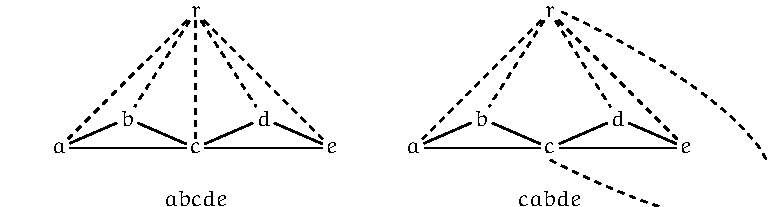
\includegraphics[scale=.9]{figures/t_subtle}
    \caption[Outerplanar embedding representing different symmetric orders]{The outerplanar embedding  
    represents the vertex orders in both $[abcde]$ and~$[cabde]$. The symmetric orders $[abcde]$ and~$[cabde]$ correspond to different edge orders around~$r$ in the extended graph.}
    \label{figure:subtle}
\end{figure}
    
Now we choose~$r$ as last vertex in the leaf-to-root order of the planarity algorithm.
Since $G$~is connected, the scheme above yields a single \PQ-tree~$T$ representing all
extendible planar embeddings of~$G$ (as possible orders of the half-embedded edges~$\{r, v\}$ for~$v\in V(G)$)  at its penultimate step. By the argument above, every such embedding
is outerplanar. Also, $T$~not only gives the orders of the half-embedded edges
but all vertices of~$G$ since~$r$ is adjacent to every other vertex, \ie every vertex of~$G$ is 
the endpoint of exactly one half-embedded edge. 

A subtle distinction is still noteworthy, although it does not present any problems
for the algorithm. When
walking around the outer boundary of an outerplanar embedding in clockwise or counter-clockwise
direction, we can meet a vertex twice. Thus, the outerplanar embedding in \myref{figure:subtle},
for example, can yield the total orders in both $[abcde]$ and~$[cabde]$; yet these orders belong
to different planar embeddings of the extended graph.

In conclusion, there is a \PQ-tree from which we can read all valid outerplanar embeddings (page embeddings). 
This \PQ-tree can be computed in linear time as shown by Haeupler and Tarjan~\cite{Haeupler08}.
%For~$C_4$ this is illustrated in \myref{figure:connected}.

\begin{lemma}\label{lemma:one-page}
Let~$G = (V, E)$ be a connected graph. Then we can compute a \PQ-tree representing all valid
orders of the vertices~$V$ in a page embedding of~$G$ in $\OO\bigl(|V|\bigr)$~time.
\end{lemma}

To get the set of valid book orders, all that remains to be done is to intersect the
\PQ-trees we get. Say we want to intersect the \PQ-trees~$S$ and~$T$ on the same leaves. Let~$v$
be an inner node of~$S$ and~$e$ one of its incident edges going to a child~$w$ of~$v$.
Then the leaves $C(w)$~that have~$w$ as ancestor appear consecutively in any order $\pi \in \pi(S)$.
Additionally, if~$v$ is a \Q-node and $e'$ is a consecutive edge of~$e$ going from~$v$ to~$w'$, then the
leaves $C(w) \cup C(w')$ also appear consecutively in any $\pi \in \pi(S)$. On the other hand,
any order fulfilling these constraints is in~$\pi(S)$. That is, we can get a tree
representing $\pi(S) \cap \pi(T)$ by applying the reductions just described to the tree~$T$.
A trivial implementation of this approach would need a quadratic number of reductions, but Booth described in his Ph.\,D. thesis~\cite{Booth75}
how to reduce the cost of intersection to linear time.

Now that we are able to intersect \PQ-trees, we can summarise the linear-time solution
of \probBookConnected.

\begin{theorem}
\probBookConnected can be solved in linear time.
\label{theorem:connected}
\end{theorem}
\begin{myproof}
Let~$(V, E_1,\dotsc, E_k)$ be the \probBookConnected instance.
First construct the $k$ \PQ-trees~$T_1,\dotsc, T_k$ representing all valid page
embeddings of the corresponding graphs~$(V, E_1), \dotsc, (V,E_k)$, each in~$\OO\bigl(|V|\bigr)$. Then consecutively
intersect $T_1$ with $T_2,\dotsc, T_k$ using time~$\OO\bigl((k - 1)|V|\bigr)$, yielding the
\PQ-tree~$T$ representing all valid solutions of the instance. The instance
possesses a solution if and only if~$T \ne \varepsilon$, which can be decided in constant time.
All in all, we need $\OO\bigl(k|V|\bigr)$~time.
\end{myproof}

\paragraph{Outlook}

When the graphs on the pages are not connected, we also get \PQ-trees for the valid orders of each of their components. That is, we have a set of \PQ-trees and must decide whether
they possess a common order in order to solve the book embedding problem. The hurdle is that the trees do not need to have the same leaves. 

Bl\"asius and Rutter~\cite{Blasius11} considered a more general variant of this \PQ-tree intersection problem, called \probPQ. They showed the
\NP-completeness of \probPQ for an unbounded number of trees. 
%As noted in \myref{section:np-complete}, we, similarly, only showed that \probBook
%is \NP-complete when the number of pages is unbounded. 
Investigating restrictions of \probPQ
may help us deal with the book embedding problem, but we are not sure how.
%By the reduction above, we can
%improve this to a constant number of pages if we manage to prove the \NP-completeness
%of \probPQ for a constant number of trees. Therefore, investigating \probPQ is one approach for extending
%our results, but it is---in our opinion---not promising since
%\probPQ is not a problem of significantly simpler form than \probBook.
\section{Disjoint perfect matchings}

\begin{frame}{Disjoint perfect matchings as pages}

%Take disjoint perfect matchings as pages.
\newProb{\probMatching}
{Disjoint perfect matchings $E_1,\dotsc, E_k$ on a vertex
set $V$.}{Is there a book embedding of $(V, E_i)$?}

\begin{theorem}
Necessary: $G := (V, E_1 \cup \dotsb \cup E_k)$ is bipartite.
\end{theorem}

\begin{overprint}
\onslide<1>
\begin{itemize}
\item Even number of vertices between adjacent vertices in valid order
\begin{figure}
\centering

\resizebox{0.6\textwidth}{!}{
\begin{tikzpicture}
\node (v) {v};
\node[right of=v,node distance=7em] (nw) {$n_i(w)$};
\node[right of=nw,node distance=7em] (w) {$w$};
\node[right of=w,node distance=7em] (nv) {$n_i(v)$};

\draw (v) edge[bend left] (nv);
\draw (nw) edge[bend left] (w);

/* v to n1 */
\draw[decoration={brace},decorate,thick] ($ (nv) + (-1.2em, -1em) $) -- ($ (v) + (0.5em,-1em) $);
\node[text centered] at ($ 0.5*($(nv) + (v)$) + (-0.25em, -2em) $) {even};

\node[text centered] at ($ 0.5*($(v) + (nw)$) + (0.25em, 0)$) {\dots};
\node[text centered] at ($ 0.5*($(nw) + (w)$) + (0.25em, 0)$) {\dots};
\node[text centered] at ($ 0.5*($(w) + (nv)$) + (0.25em, 0)$) {\dots};
\end{tikzpicture}
}
\end{figure}
\end{itemize}

\onslide<2>
\begin{itemize}
\item Even number of vertices between adjacent vertices in valid order
\item[$\Rightarrow$] Vertices with even and odd indexes form bipartition
\end{itemize}
\end{overprint}

\end{frame}

\begin{frame}{Bipartite examples}
\begin{figure}[\placement]
\centering

\scalebox{1.3}{%
\begin{tikzpicture}

\node (l1) {{\relscale{0.5}$l_0$}};
\node[right of=l1,node distance=6em] (r1) {{\relscale{0.5}$r_0$}};
\node[below of=l1] (l2) {{\relscale{0.5}$l_1$}};
\node[right of=l2,node distance=6em] (r2) {{\relscale{0.5}$r_1$}};
\node[below of=l2] (l3) {{\relscale{0.5}$l_2$}};
\node[right of=l3,node distance=6em] (r3) {{\relscale{0.5}$r_2$}};
\node[below of=l3] (l4) {{\relscale{0.5}$l_3$}};
\node[right of=l4,node distance=6em] (r4) {{\relscale{0.5}$r_3$}};

\draw (l1) edge (r1);
\draw (l2) edge (r2);
\draw (l3) edge (r3);
\draw (l4) edge (r4);
\draw[edge1] (l1) edge (r2);
\draw[edge1] (l2) edge (r3);
\draw[edge1] (l3) edge (r4);
\draw[edge1] (l4) edge (r1);
\draw[edge2] (l1) edge (r3);
\draw[edge2] (l2) edge (r4);
\draw[edge2] (l3) edge (r1);
\draw[edge2] (l4) edge (r2);
\draw[edge3] (l1) edge (r4);
\draw[edge3] (l2) edge (r1);
\draw[edge3] (l3) edge (r2);
\draw[edge3] (l4) edge (r3);
\end{tikzpicture}}
\end{figure}

$k$ pages: Take the partition $E_i := \bigl\{\{l_j, r_{(j + i)\bmod{k}}\}: j \in \range{k-1}\bigr\}$ of $K_{k,k}$ 
\end{frame}

\begin{frame}{Bipartite counterexamples}
\begin{figure}[\placement]
\centering

\scalebox{1.3}{%
\begin{tikzpicture}

\node (l1) {{\relscale{0.5}$l_1$}};
\node[right of=l1,node distance=6em] (r1) {{\relscale{0.5}$r_1$}};
\node[below of=l1] (l2) {{\relscale{0.5}$l_2$}};
\node[right of=l2,node distance=6em] (r2) {{\relscale{0.5}$r_2$}};
\node[below of=l2] (l3) {{\relscale{0.5}$l_3$}};
\node[right of=l3,node distance=6em] (r3) {{\relscale{0.5}$r_3$}};
\node[below of=l3] (l4) {{\relscale{0.5}$l_4$}};
\node[right of=l4,node distance=6em] (r4) {{\relscale{0.5}$r_4$}};

\draw (l1) edge (r1);
\draw (l2) edge (r2);
\draw (l3) edge (r3);
\draw (l4) edge (r4);
\draw[edge1] (l1) edge (r2);
\draw[edge1] (l2) edge (r1);
\draw[edge1] (l3) edge (r4);
\draw[edge1] (l4) edge (r3);
\draw[edge2] (l1) edge (r3);
\draw[edge2] (l3) edge (r1);
\draw[edge2] (l2) edge (r4);
\draw[edge2] (l4) edge (r2);
\draw[edge3] (l1) edge (r4);
\draw[edge3] (l4) edge (r1);
\draw[edge3] (l2) edge (r3);
\draw[edge3] (l3) edge (r2);
\end{tikzpicture}}
\end{figure}

$k \geq 4$ pages: Partition $K_{k,k}$ into disjoint perfect matchings that contain
this counterexample
\end{frame}

\begin{frame}{Bipartite counterexample for three pages}
Smallest counterexample where two of the matchings form a cycle\vspace{-1em}
\begin{figure}[\placement]
\centering
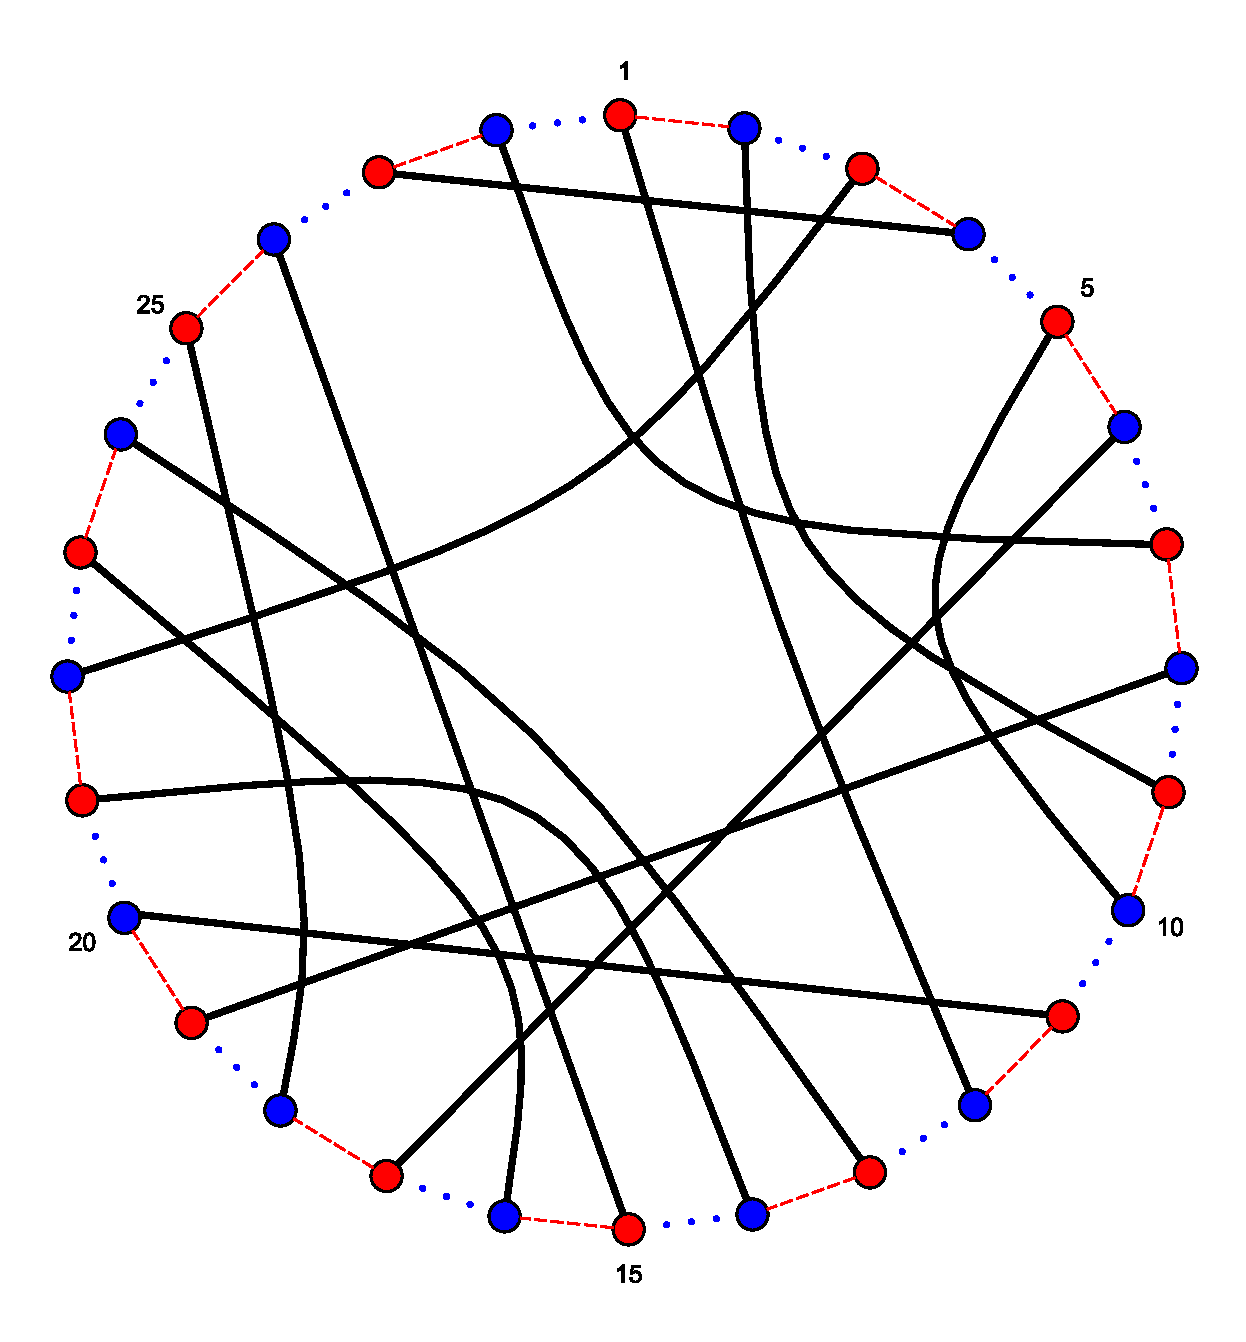
\includegraphics[width=0.5\textwidth]{../thesis/figures/two_cycles.eps}
\end{figure}
\vspace{-1em} Smallest unrestricted counterexample: $20 \leq n \leq 28$
\end{frame}

\resultFrame{4}
\section{\PQ-tree on the Vertices}
\label{section:trees}

\noindent 

Besides demanding that pages have a special structure, as we have
done in the preceding sections, we may
restrict the order of the vertices to a subset
of the symmetric group~$S_n$ that we can, hopefully, work with more easily. 

Angelini et.\,al.~\cite{angelini11} showed that \SEFECON~(see page~\pageref{prob:sefecon}) can be reduced to a 2-page embedding problem where the vertex order comes from a \PT-tree.

For this reason it is useful to restrict the permutations with \PQ-trees. That is, we do
the very opposite of \myref{section:connected} and start with a \PQ-tree
instead of getting a tree that represents the possible book embeddings.

\begin{figure}[\placement]\centering
    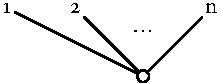
\includegraphics{figures/t_pq-all}
    \caption[\PQ-tree that represents all permutations]{A \PQ-tree that represents all permutations of $\range{n}$.}
    \label{figure:pq-all}
\end{figure}

A general~\PQ-tree does not really help
since the \PQ-tree in \myref{figure:pq-all} (a single \PT-node) represents all permutations of $\range{n}$,
\ie the problem does not get easier.

Thus, we have to narrow down the possible permutations even more. In this section we only consider
\Q-trees and show that \probQTree, which is \probBook restricted to~\Q-trees,
can be solved in quadratic time. In order to do this, we provide a reduction of the problem to~\probTwoSat, the problem of checking a 2-CNF formula for satisfiability. 
The \probTwoSat problem is solvable in linear time as first shown by Krom~\cite{Krom67}.

\newProb{\probQTree}{A \probBook instance $I$ with vertices $V$ and a \Q-tree~$T$ with leaves~$V$.}{Is there a total order $<\,\in \pi(T)$ solving $I$?}
\newProb{\probPTree}{A \probBook instance $I$ with vertices $V$ and a \PT-tree~$T$ with leaves~$V$.}{Is there a total order $<\,\in \pi(T)$ solving $I$?}
\newProb{\probTwoSat}{A 2-\CNF Boolean formula \bool{f}.}{Is~\bool{f} satisfiable?}

\Q-Trees are exactly the wrong type of trees
compared to the reformulation of the \SEFECON problem by Angelini et.\,al.~\cite{angelini11} since \Q-nodes vastly restrict the possible
permutations and are significantly easier to handle than \PT~nodes. This
section, therefore, only solves \SEFECON if the \PT-tree of the equivalent \probPTree instance is also a \Q-tree, \ie if the \PT-tree is a binary tree.

We first investigate what possible configurations of the leaves the book constraints 
lead to when we take the \Q-tree~$T$ into account. Then we show how these configurations
can be expressed with a 2-\CNF formula.

\paragraph{Possible configurations resulting from a book constraint}

\begin{figure}[\placement]\centering
    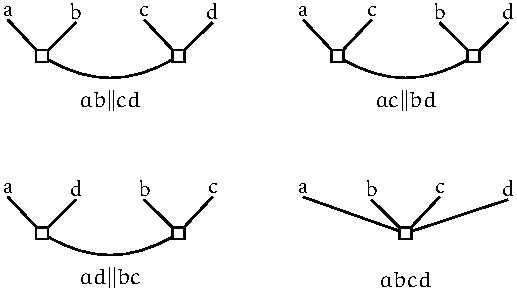
\includegraphics{figures/t_topo1}
    \caption[Topologies of four leaves]{The possible topologies of four leaves $a, b, c, d$ in a tree.}
    \label{figure:topo1}
\end{figure}


We first show that the book embedding restrictions for two edges $\{a, b\}$ and $\{c, d\}$
can be translated directly to restrictions on the $Q$-tree.
Before we start with this translation, however, we list some conventions. The \Q-tree is called $T$ and has leaves~$V$. Furthermore, let $t(M)$ be the smallest subtree of~$T$ containing~$M$ and let~$r(M)$ be its root for any~$M \subseteq V$.
Also remember that we assumed  in \myref{section:total-ordering} that any two edges we consider the book constraint for are independent.

%Consider the tree~$t(M)$ for~$M := \{a, b, c, d\}$.

We want to distinguish cases based on which two leaves in~$M := \{a, b, c, d\}$ can be separated from the others. These possible \emph{topologies of $M$ in~$T$} are depicted in \myref{figure:topo1}.
For example, we have~$ab||cd$ if there is an edge~$e \in E(T)$ such that $a$ and~$b$ are
in one component of~$T \setminus e$ while $c$ and~$d$ are in the other component, \ie
$a$ and~$b$ can be separated from $c$ and~$d$.
The topologies for $ac||bd$ and~$ad||bc$ are defined analogously. If no two vertices in~$M$ can be separated from the other
two (all pairs of vertices in~$M$ have the same lowest common ancestor) we say that the topology~$abcd$ occurs. 

%Thus, $t(M)$ has one of the trees in \myref{figure:topo1} as a
%topological minor, \ie the leaves $a$, $b$, $c$ and $d$ can appear
%in only a small number topological configurations. (Note that we do not take into consideration that the tree is rooted and ordered.) We call these configurations ``topologies'' below.

Depending on which of the topologies occurs, we can map the constraint from \myref{lemma:constraints} to a Boolean formula on the order~$<$ of the vertices~$V$.

\paragraph{Case 1: ab||cd}

Since $\{a, b\}$ and $\{c, d\}$ are in disjoint subtrees and the vertices of
a subtree are consecutive in every permutation $\pi(T)$, all tree orders
fulfil the book constraint. Thus, the constraint is mapped to the Boolean expression \bool{true}.

\paragraph{Case 2: ac||bd}

\begin{figure}\centering
    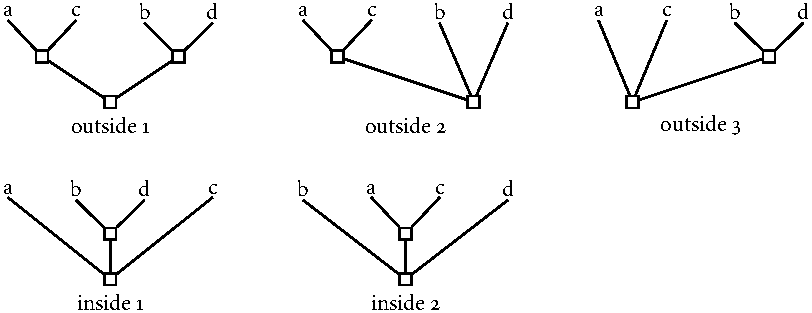
\includegraphics[scale=.9]{figures/t_order_ab_cd}
    \caption[Trees for $ac||bd$]{The possible trees corresponding to $ac||bd$.}
    \label{figure:order_ab_cd}
\end{figure}
\begin{figure}\centering
    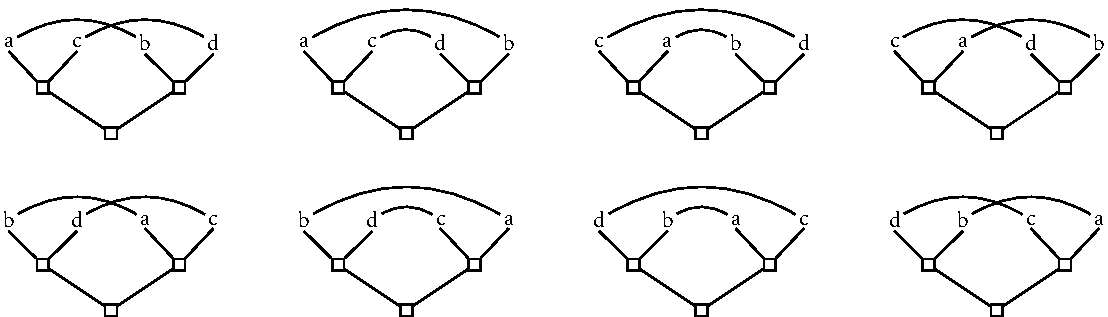
\includegraphics[width=\textwidth]{figures/t_topo_ac_bd}
    \caption[Outside 1 tree orders]{The tree orders for the case outside 1.}
    \label{figure:topo_ac_bd}
\end{figure}
\begin{figure}\centering
    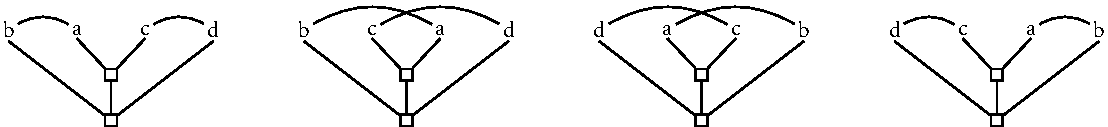
\includegraphics[width=\textwidth]{figures/t_topo_b_ac_d}
    \caption[Inside 1 tree orders]{The tree orders for the case inside 1.}
    \label{figure:topo_b_ac_d}
\end{figure}

In this case we search through the possible trees to determine the resulting
\probTwoSat formula. To do this systematically, we have to take into account that~$T$ is ordered and rooted and determine what the tree can look like. 

Thus, we further split this case into sub-cases based on whether the vertices $a$ and~$c$ are between $b$ and~$d$ (inside), $b$ and~$d$ are between $a$ and~$c$ (inside) or no two vertices in~$M$ are between the vertices they are separated from (outside). Note that $a$ and~$c$ are between $b$ and~$d$
for all orders in~$\pi(T)$ if they are between $b$ and~$d$ for one order in~$\pi(T)$ since~$T$
is a \Q-tree.

In the outside case, the
possible permutations also depend on how the roots of the subtrees $t(a, c)$ and $t(b, d)$ are related,
\ie whether one appears as a child of the other. The possible tree structures are depicted
in \myref{figure:order_ab_cd}.  
%We especially need not fix any portion of the order.

For each tree, we can exhaustively search through the orders of the leaves~$M$ the tree permits. For the 
case outside~1 these orders are portrayed in \myref{figure:topo_ac_bd}. We observe that the
valid orders are exactly the orders with $a < c \Leftrightarrow d < b$. The other two outside
cases can be handled similarly. Both of them again yield $a < c \Leftrightarrow d < b$.

For the inside cases we do the same. The possible orders of the case inside~1 are depicted in \myref{figure:topo_b_ac_d}. We can infer the
inverse $a < c \Leftrightarrow b < d$ for both inside cases. 

\paragraph{Case 3: ad||bc}

As in case~2, we either get $a < d \Leftrightarrow b < c$ or
$a < d \Leftrightarrow c < b$.

\paragraph{Case 4: abcd}

Let~$r$ be the common root $r(a, b, c, d)$ of $M := \{a, b, c, d\}$. The tree~$T$
represents two permutations of $M$ since the children of the \Q-node~$r$ can
only be reversed. If the book constraint is valid in a permutation of~$M$, it is also valid in the
mirror image of the permutation. Therefore, the book constraint may be valid in none or both of the two possible permutations. That is, we get either \bool{true} or
\bool{false} as constraint.

\paragraph{Mapping \probBook to \probTwoSat}

We now show how the resulting Boolean expressions can be mapped to \probTwoSat formulae.
To do so we fix a reference orientation of the inner nodes of~$T$.
For each $\pi \in \pi(T)$ and every inner node $v$ in $T$, we can say whether
we got $\pi$ as a permutation in~$\pi(T)$ by giving~$v$ the reference orientation or not.
Introduce a Boolean variable $o_v$ that stands for~$v$ being in reference orientation.

By the construction above, a book constraint for two edges yields one of the following Boolean expressions dependent on the structure of~$T$.

\begin{enumerate}
  \item A trivial expression \bool{true} or \bool{false}. (from cases~1 and~4)
  \item A fixed order of two leaves $v$ and~$w$ which is the same
  as fixing the order of their root~$r := r(v, w)$. Thus, we get
  $o_r$ or $\lnot o_r$. (from case~4)
  \item A connection between the orders of the leaves $a$, $b$ and $c$, $d$
  that are located in disjoint subtrees. This is the same as tying the
  orders of the roots $r := r(a, b)$ and $s := r(c, d)$ together.
  We get either $o_r \Leftrightarrow o_s \equiv (\lnot o_r \lor o_s) \land (\lnot o_s \lor o_r)$
  or $o_r \Leftrightarrow \lnot o_s \equiv (\lnot o_r \lor \lnot o_s) \land (o_s \lor o_r)$. (from cases~2 and~3)
\end{enumerate}

Thus, we can reduce \probQTree to determining whether a set of 2-\CNF expressions
is consistent with a \Q-tree structure. But since the inner nodes of a \Q-tree can be flipped completely independently of each other, the consistency with the \Q-tree structure does not
impose any extra restrictions. That is, \probQTree can be mapped to checking
a \probTwoSat formula for consistency (satisfiability).


%\newProb{\probQTreeSat}{A \Q-tree $T$ and a 2-\CNF expression $m$ on $\{o_v\colon \text{$v$ 
%is inner node of $T$}\}$ with $o_v$~signifying that the node~$v$ is ordered as in the initial tree.}{Is there a permutation in~$\pi(T)$ where~$m$ is satisfied?}

We now see how the reduction from \probQTree to \probTwoSat above can be 
implemented in qua\-dratic time.

\begin{lemma}
\label{lemma:q-tree-redux}
\probQTree can be reduced to \probTwoSat in quadratic time.
%A $\probQTree$~instance  can be reduced
%to a $\probTwoSat$ instance in $\OO\bigl(|T| + |E_1|^2 + \dotsb + |E_k|^2\bigr)$~time.
\end{lemma}
\begin{myproof}
Let $\bigl((V, E_1),\dotsc, (V, E_k), T\bigr)$ be an instance of $\probQTree$.
We can map the book constraints for each pair $e_1, e_2 \in E_i$ of edges for all
$i \in \range{k}$ to a 2-\CNF formula with the construction above.

Let's investigate how this can be done efficiently. Our goal is
to map each book constraint resulting from a pair of edges to a 2-\CNF formula in constant
time after a linear time precomputation. 

We assume $V = \range{n}$ and that each inner node of the tree~$T$ 
contains a pointer to its parent and an (ordered) list of its children.
Furthermore, let~$r$ be the root of~$T$.

%\begin{Ualgorithm}[\placement]
%\caption{Class for rooted, ordered trees}\label{alg:tree}
%\DontPrintSemicolon
%
%\SetKwFor{Class}{class}{}
%
%\SetKwFunction{Tree}{Tree}
%\SetKwFunction{PTree}{Pointer to Tree}
%\SetKwFunction{VTree}{Vector of pointers to Tree}
%\SetKwFunction{MyInt}{Integer}
%
%\Class{\Tree}{parent: \PTree\;children: \VTree}
%\end{Ualgorithm}

To determine the topology of a quadruple of leaves, we need to know
the lowest common ancestor of certain pairs of nodes and their initial order.

The first problem has been studied extensively. Harel and Tarjan~\cite{Harel84} showed
the surprising result that lowest common ancestor queries can be answered in constant
time after a linear time precomputation, although their algorithm was too complicated to be implemented
effectively. Farach and Colton~\cite{Farach00} presented a far simpler variant of this
algorithm that is used in practice. We assume in the following that the precomputation has 
been done and that \algoFont{LCA($x$, $y$)} gives the lowest common ancestor of~$x$ and~$y$ in~$\OO(1)$ time.

For the second problem, we can precompute the index array~\algoFont{idx} of~$V$ that maps each
leaf~$V$ to its index in the reference orientation of~$T$. This can be accomplished in linear time by a simple depth-first search. 

%At each step,
%we know the index the leaves in the current subtree start with. We recurse on the children
%of the current node in order and update the starting index accordingly. When we arrive at a
%leaf, we know that its index is the current starting index, which is given as a parameter. The initial
%call is~\algoFont{ComputeIndex$(r, 1)$}.
%
%\begin{Ualgorithm}[\placement]
%\caption[Computing the index array]{Computing the index array: \algoFont{ComputeIndex}}\label{alg:index}
%
%\SetKwFunction{Tree}{Tree}
%\SetKwFunction{ComputeIndex}{ComputeIndex}
%\SetKwFunction{size}{size}
%\SetKwFunction{content}{idx}
%\SetKwFunction{children}{children}
%
%\SetKwData{T}{T}
%\SetKwData{firstIdx}{s}
%\SetKwData{lastIdx}{e}
%\SetKwData{idx}{idx}
%\SetKwData{mycnt}{i}
%
%\KwIn{Tree $T$, starting index $s$}
%\KwOut{Ending index $e$}
%
%\BlankLine
%\tcp{Is $T$ leaf?}
%\If{$\T.\children.\size = 0$}{
%$\lastIdx \leftarrow \firstIdx$ \;
%$\idx[\T.\content] \leftarrow \firstIdx$
%}
%\Else {
%	\tcp{Recurse and update indexes}
%	\For{$\mycnt \leftarrow 1$ to $\T.\children.\size$}{
%		$\firstIdx \leftarrow \ComputeIndex(\T[\mycnt], \firstIdx) + 1$
%	}
%}
%\end{Ualgorithm}

Before we begin with the actual translation, we need another helper function \algoFont{Leaf-Order($a$,$b$)} that translates a statement
of the form~$a < b$ for leaves $a, b \in V$ into a literal on the variable~$o_r$ 
where $r = \algoFont{LCA}(a, b)$. If $\algoFont{idx[a]} < \algoFont{idx[b]}$, then~$r$ has reference orientation and the result is~$o_r$. Otherwise, the result is~$\lnot o_r$. This decision can obviously
can be made in $\OO(1)$~time.

%\begin{Ualgorithm}[\placement]
%\caption[Literal for leaf order]{A literal for a given leaf order: $\algoFont{Leaf-Order}$}\label{alg:lca}
%
%\KwIn{Leaves $a, b \in V$}
%\KwOut{A Boolean formula representing $a < b$}
%
%\SetKwFunction{LCA}{LCA}
%
%\SetKwData{firstPar}{a}
%\SetKwData{secondPar}{b}
%\SetKwData{idx}{idx}
%
%\BlankLine
%$r \leftarrow \LCA(\firstPar, \secondPar)$ \;
%\If{$\idx[\firstPar] < \idx[\secondPar]$}{
%	\KwRet $o_r$
%}
%\Else{
%	\KwRet $\lnot o_r$
%}
%\end{Ualgorithm}

We now have everything we need to translate book constraints into
Boolean formulae. The direct formalisation of the construction
above is given in \myref{alg:translate}. It returns
a Boolean formula for a pair of edges $\{a, b\}$ and~$\{c, d\}$
in~$\OO(1)$. Note that we can test whether the order~\algoFont{idx} fulfils
the book constraint in line~9 in~$\OO(1)$ time since only the relative
order of $a$, $b$, $c$ and $d$ is relevant.

In the algorithm, the Boolean formulae are not given in conjunctive normal
form for the sake of clarity. If we want \CNF~formulae, we can statically replace
the Boolean formulae in \myref{alg:translate} by their \CNF~equivalents.


\SetAlFnt{\footnotesize\sffamily}
\begin{Ualgorithm}[\placement]
\caption[Translating the book constraint in $\OO(1)$]{Translating the book constraint in $\OO(1)$ }
\label{alg:translate}

\SetKwFunction{LCA}{LCA}
\SetKwFunction{LeafOrder}{Leaf-Order}

\SetKwData{pa}{a}
\SetKwData{pb}{b}
\SetKwData{pc}{c}
\SetKwData{pd}{d}
\SetKwData{idx}{idx}

\KwIn{Two edges $\{\pa, \pb\}$ and $\{\pc, \pd\}$}
\KwOut{A Boolean formula representing the book constraint for the two edges}

\BlankLine

\tcp{Independent edges?}
\If{$|\{\pa, \pb, \pc, \pd\}| = 4$}{
	$r_1 \leftarrow \LCA(\pa, \pb)$ \;
    $r_2 \leftarrow \LCA(\pa, \pc)$ \;
	$r_3 \leftarrow \LCA(\pa, \pd)$ \;
	$r_4 \leftarrow \LCA(\pb, \pc)$ \;
	$r_5 \leftarrow \LCA(\pb, \pd)$ \;
	$r_6 \leftarrow \LCA(\pc, \pd)$ \;
	\If{all~$r_i$ are the same for~$i \in \range{6}$}{
		\tcp{$abcd$}
%		$x \leftarrow \text{leaf with smallest \idx among \pa, \pb, \pc and \pd}$ \;
%		$y \leftarrow \text{leaf with largest \idx among \pa, \pb, \pc and \pd}$ \;
		\If{Order \idx fulfils book constraint}{
			\KwRet $true$
		}
		\Else{
			\KwRet $false$
		}
	} \ElseIf{$\LCA(r_2, r_5)$ is not equal to $r_2$ or $r_5$}{
		\tcp{$ac||bd$}
		\If{$\idx[\pa]$ between $\idx[\pb]$ and $\idx[\pd]$}{
			\KwRet $\LeafOrder(\pa, \pc) \Leftrightarrow \LeafOrder(\pb, \pd)$
		}
		\Else {
			\KwRet $\LeafOrder(\pa, \pc) \Leftrightarrow \LeafOrder(\pd, \pb)$
		}
	} \ElseIf{$\LCA(r_3, r_4)$ is not equal to $r_3$ or $r_4$}{
	    \tcp{$ad||bc$}
	    \If{$\idx[\pa]$ between $\idx[\pb]$ and $\idx[\pc]$}{
			\KwRet $\LeafOrder(\pa, \pd) \Leftrightarrow \LeafOrder(\pb, \pc)$
		}
		\Else {
			\KwRet $\LeafOrder(\pa, \pd) \Leftrightarrow \LeafOrder(\pc, \pb)$
		}
	} \Else {
	    \tcp{$ab||cd$}
		\KwRet $true$
	}
}
\Else{
	\KwRet $true$
}
\end{Ualgorithm}

All in all, we need~$\OO\bigl(|T|\bigr)$ time for the precomputation and
$\OO(1)$~time for each of the~$\OO\bigl(|E_1|^2+\dotsb+|E_k|^2\bigr)$ book constraints.
Thus, the reduction to \probQTreeSat takes $\OO\bigl(|T| + |E_1|^2 + \dotsb + |E_k|^2\bigr)$~time.\qedhere
%We need to determine the topological structure of each of the
%$|E_1|^2 + \cdots + |E_n|^2$ edge pairs $e_1$ and $e_2$. This
%can be done in~$\OO(|T|)$ by following a path from a vertex of $e_1$ to the root
%if we have a bit-field of length $\OO(|V|)$ for each inner node $v$~of~$T$ from which we
%can determine, whether a leaf is contained in the subtree rooted at~$v$. The bit-field
%can be recursively precomputed in time $\OO(|T|^2|V|)$.

%Thus, the reduction to \probQTreeSat takes $\OO(|T|\cdot(|E_1|^2 + \cdots + |E_n|^2 + |V||T|))$~time
\end{myproof}

%The problem~\probQTreeSat is clearly efficiently solvable.

%\begin{lemma}
%An instance~$(T, m)$ of \probQTreeSat can be solved in $\OO\bigl(|m|\bigr)$.
%\end{lemma}
%\begin{myproof}
%The inner nodes of~$T$ can be flipped completely independently of each other,
%\ie there are no constraints on the~$o_v$ except the ones given in~$m$.
%Since~$m$ is a 2-\CNF expression, checking it for consistency (satisfiability)
%can be done in $\OO\bigl(|m|\bigr)$ as first shown by Krom~\cite{Krom67}.
%\end{myproof}

Since \probTwoSat is solvable in linear time, we conclude that \probQTree can be solved in quadratic time.

\begin{theorem}
\label{theorem:q-tree-book}
\probQTree can be solved in quadratic time.
\end{theorem}
\begin{myproof}
Let $\bigl((V, E_1),\dotsc, (V, E_k), T\bigr)$ be an instance of $\probQTree$.
We saw that the reduction to \probTwoSat takes $\OO\bigl(|T| + |E_1|^2 + \dotsb + |E_k|^2\bigr)$ time
in \myref{lemma:q-tree-redux}. For each pair of edges $e_1, e_2 \in E_i$ where $i \in \range{n}$ we get a 2-\CNF expression of length $\OO(1)$. Since \probTwoSat is solvable in linear
time as first shown by Krom~\cite{Krom67}, we, therefore, need $\OO\bigl(|E_1|^2 + \dotsb + |E_n|^2\bigr)$~time to solve the resulting \probTwoSat problem.
Altogether, we need $\OO\bigl(|T| + |E_1|^2 + \dotsb + |E_k|^2\bigr)$ time.
\end{myproof}

We have assumed $|E_i| \le 2|V|-3$ for all~$i \in \range{k}$ at the
start of \myref{ch:preliminaries} since the pages
have to be outerplanar to be embeddable. Furthermore, the \Q-tree 
has fewer inner nodes than its number of leaves~$|V|$ since each inner node
has at least two children.
That is, we can rewrite the time as
$\OO\bigl(|T| + |E_1|^2 + \dotsb + |E_k|^2\bigr) = \OO\bigl(|V| + k(2|V|-3)^2\bigr) = \OO\bigl(k|V|^2\bigr)$.

\paragraph{Outlook}

So book embedding is solvable in quadratic time if we constrain the vertex order by a \Q-tree. But what if we have a \PT-tree as in the
reformulation of \SEFECON? We have already seen in \myref{figure:pq-all} that this
restriction cannot make the problem simpler than the general book embedding problem. Furthermore, we cannot directly generalise our construction since the answer to ``What permutation of the children of a \PT-node occurs?'' cannot simply be modelled by a Boolean variable.
%for example, the sub-argument for $ac||bd$ depends on us being able to distinguish between the inside
%and outside cases. If the common root $r := r(a, b, c, d)$ were a \PT-node, the tree would
%allow permutations with $ac$ between~$bd$ and permutations where this is not the case, \ie there are %valid
%orders with $a < c \land b < d$ and ones with $a < c \land d > b$. This means that we cannot simply
%model the book constraint by looking at how~$r$ is flipped.
That is, \probPTree remains an
interesting open problem.
\section{Multiple Spines}\label{section:multi_spine}

In the previous sections we showed how \PQ-trees relate
to book embeddings. On the one hand they can help to solve
the problem for connected graphs on the pages and on the other hand
we can restrict the orders of the vertices with a \PQ-tree, yielding
an interesting modification to book embedding.

\begin{figure}[\placement]\centering
    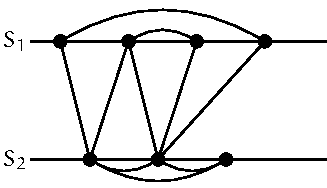
\includegraphics{figures/t_two_spines}
    \caption[Two-spine drawing]{A two-spine drawing.}
    \label{figure:two_spines}
\end{figure}

We now consider another variation on book embedding which 
will turn out to be a special case of the latter application of \PQ-trees.
It is a generalisation of the 2-page case that uses not just one spine but several parallel
spines~(lines) $S_1$, \dots, $S_k$. In the following considerations we always assume
that $S_i$~is above~$S_{i+1}$ for all $i\in\range{k-1}$.
We want to planarly draw one graph above~$S_1$,
one between~$S_i$ and $S_{i+1}$ for each $i \in \range{k-1}$ and one
below~$S_k$, as depicted in \myref{figure:two_spines} for
two spines. This problem is motivated by \emph{level planarity} which
is the same problem without the \emph{caps}, the graph above~$S_1$ and
the graph below~$S_k$.
The level planarity problem was first introduced by Tomii~et.~al.~\cite{Tomii77}. 
Jünger, Leipert and
Mutzel presented an algorithm that checks for level planarity in linear time~\cite{Junger99}.

In this section we show that the multiple spine problem is equivalent to a 2-page book embedding problem constrained by a special \PT-tree, but do not manage to give an efficient algorithm
it. Still, this reinforces our belief that \probPTree is an interesting problem.

Let the spines always be~$S_i = \SR \times \{-i\}$. We now formally define
the problem. It will turn out to be convenient to formally use directed edges pointing downward for the edges between the spines, but we still understand and draw these edges as undirected edges.

\newProb{\probMul}{Vertex sets~$V_1$, \dots, $V_k$ and
edge sets $E_0 \subseteq \binom{V_1}{2}$, $E_1 \subseteq V_1\times V_2$,
\dots, $E_{k-1} \subseteq V_{k-1} \times V_k$, $E_k \subseteq \binom{V_k}{2}$.}{Is there
a planar drawing of $(V_1 \cup \dotsb \cup V_k, E_0 \cup \dotsb \cup E_k)$ such that
a vertex in~$V_i$ lies on~$S_i$ for all~$i \in \range{k}$, edges do not cross a spine,
the edges in~$E_0$ lie completely above~$S_1$ and the edges in~$E_k$ lie completely below~$S_k$?}

Tomii~et.~al.~\cite{Tomii77} showed that the 2-level planar graphs are exactly the forests
of caterpillars. Recall that a \emph{caterpillar} is a tree all of whose vertices are on
a central path or one edge away from it. Therefore, each of the graphs~$(V_i \cup V_{i+1}, E_i)$ for~$i \in \range{k-1}$ has to be a forest, \ie we find~$|E_i| = |V_i| + |V_{i+1}| - l$ if this
forest has $l$~components. That is, as in the case of page embedding the number of edges is again linear in
the number of vertices. Thus, the size of a \probMul~instance is in~$\OO\bigl(|V_1| + \dotsb + |V_k|\bigr)$.

\begin{figure}[\placement]\centering
    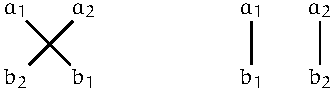
\includegraphics{figures/t_level_order}
    \caption[Level planarity is an ordering problem]{Level planarity only depends on the order of the vertices.}
    \label{figure:level_order}
\end{figure}

From \myref{lemma:constraints} we know that book embedding is essentially an ordering problem.
Similarly, consider two edges $(a_1, b_1)$ and~$(a_2, b_2)$ lying between the same two spines
and investigate how their embeddability depends on the order of their endpoints. If
$a_1$~lies left of~$a_2$ on the upper spine and $b_2$~lies left of~$b_1$ on the lower spine, then any Jordan curve from $a_1$ to~$b_1$ between the spines must intersect with any Jordan curve from $a_2$ to~$b_2$ between the spines by the Jordan curve theorem, \ie there cannot 
be a level embedding with this order. This case is depicted in \myref{figure:level_order}. Similarly,
if $a_2$~lies left of~$a_1$ and $b_1$~lies left of~$b_2$, the edges~$(a_1, b_1)$ and~$(a_2, b_2)$ also
cannot be embedded.

In any other order we can just draw a straight line for both
edges to obtain a valid embedding of the edges. After combining these observations for all pairs
of edges and taking the caps into account, we get a total order formulation of \probMul.
 
\begin{lemma}\label{lemma:multi_spine_total}
Let~$I := (V_1, \dotsc, V_k, E_0, \dotsc, E_k)$ be a \probMul instance. Then~$I$ is solvable
if any only if there is a linear order~$<_i$ on~$V_i$ for each $i \in \range{k}$ such
that the following properties hold. For all~$i \in \{1, \dots, k-1\}$ and pairs of edges~$(a_1, b_1), (a_2, b_2) \in E_i$ the order $a_1 <_i a_2 \land b_2 <_{i+1} b_1$ does not occur. Furthermore,
for $i\in\{0, k\}$ and all $\{a, b\}, \{c, d\} \in E_i$ we must not have $a <_i c <_i b <_i d$.
\end{lemma}

The order constraint for level planarity looks very similar to the book constraint,
just separated into two total orders. Indeed, if we have a \probMul instance we can find a corresponding
book embedding instance.
\begin{figure}\centering
    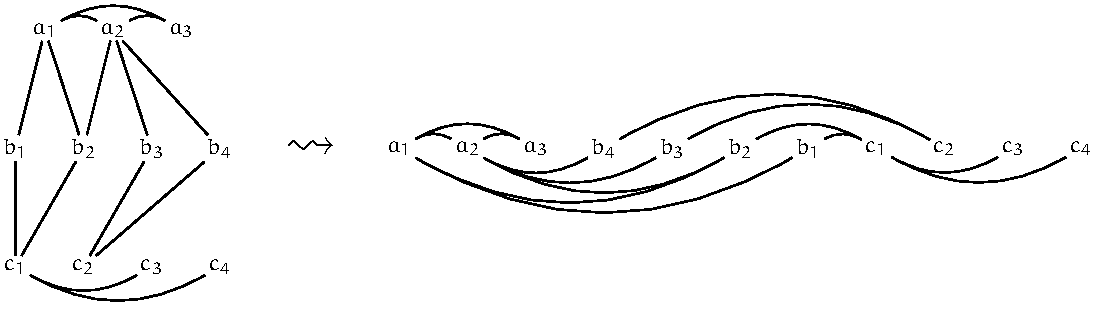
\includegraphics[width=0.9\textwidth]{figures/t_level_map}
    \caption[\probMul instance to book embedding instance]{A \probMul instance can be transformed into a 2-page book embedding instance
with separated sets of vertices.}
    \label{figure:level_map}
\end{figure}
\vskip1em
\begin{theorem}
Let~$I := (V_1, \dotsc, V_k, E_0, \dotsc, E_k)$ be a \probMul instance. We define
a corresponding 2-page book embedding instance by taking $V := V_1 \cup \dotsb \cup V_k$
as vertices and 
\begin{align*}
\widetilde{E}_1 := \bigcup_{\substack{i \in \{0, \dotsc, k\}\\ i \text{\emph{ even}}}} E_i\\
\widetilde{E}_2 := \bigcup_{\substack{i \in \{0, \dotsc, k\}\\ i \text{\emph{ odd}}}} E_i
\end{align*}
as pages. Then~$I$ is solvable if and only if~$J := (V, \widetilde{E}_1, \widetilde{E}_2)$
has a book embedding where the vertices in each~$V_i$ are consecutive.
\end{theorem}

\begin{myproof}
\begin{itemize}
\item[]
\item[``$\Rightarrow$''] Let~$<_i$ for~$i \in \range{k}$ be total orders forming a valid 
embedding of~$I$. 

Then define~$<$ on~$V$ to be the total order that first lists the
vertices of~$V_1$, then the vertices of~$V_2$, and so on. Get the inner order of the vertices
in~$V_i$ from~$<_i$ if~$i$ is even and from~$<_i$ reversed if~$i$ is odd. This
construction is illustrated in \myref{figure:level_map}.

The order~$<$ is a valid solution of the book embedding problem~$J$:
The edges in distinct edge sets~$E_i$ do not intersect by the construction of~$<$ and the definitions
of $\widetilde{E}_1$ and $\widetilde{E}_2$. Edges in~$E_0$ or~$E_k$ do not intersect since~$<_1$
and~$<_k$ are valid page embeddings for~$(V_1, E_0)$ and~$(V_k, E_k)$, respectively. Now take
two edges~$(a_1, b_1), (a_2, b_2) \in E_i$ for some~$i \in \range{k-1}$. If~$a_1 < a_2 < b_1 < b_2$
occurs, we have~$a_1 <_i a_2\;\land\;b_1 <_{i+1} b_2$, contradicting the validity of
the initial solution of~$I$. Thus, the book constraint for the two edges is fulfilled.
\item[``$\Leftarrow$''] Let~$<$ be a valid book order of~$J$ where
the sets~$V_i$ with~$i \in \range{k}$ are separated. Do the construction above in reverse, \ie
define~$<_i$ to be the restriction of~$<$ to~$V_i$ for all~$i \in \range{k}$. Additionally,
reverse~$<_i$ when~$i$ is odd.

The order~$<_i$ yields a valid embedding for~$I$: The caps already appeared in the book embedding
problem~$J$, \ie they are still valid. If~$a_1 <_i a_2\;\land\;b_2 <_{i+1} b_1$ occurs for some~$(a_1, b_1), (a_2, b_2) \in E_i$ and~$i \in \range{k-1}$, then we must have either~$a_1 < a_2 < b_1 < b_2$,
$a_2 < a_1 < b_2 < b_1$, $b_1 < b_2 < a_2 < a_1$ or~$b_2 < b_1 < a_1 < a_2$. All of these
cases contradict the book constraints.\qedhere
\end{itemize}
\end{myproof}

\paragraph{Outlook}

All in all, we see that \probMul is equivalent to a 2-page book
embedding problem where the vertex sets~$V_i$ with~$i \in \range{k}$ have to be 
separated. This separation can be modelled by a \PT-tree by introducing a \PT-node
connected to the vertices~$V_i$ for all~$i \in \range{k}$ and connecting all 
of these \PT-nodes to a single root. 

Since \probMul is an interesting problem in its own right, this leaves several
distinct possibilities for further results:
\begin{itemize}
\item Provide a polynomial time algorithm for  \probPTree and get an efficient solution of \probMul.
\item Prove the \NP-completeness of \probMul and get the \NP-completeness of \probPTree.
\item Provide a polynomial time algorithm for \probMul and get an efficient algorithm for a special case of \probPTree.
\end{itemize}
	%% conclusion.tex
%%

%% ==================
\chapter{Conclusion}
\label{ch:conclusion}
%% ==================

In this thesis we considered the book
embedding problem where the assignment of edges to pages has already been fixed.

We proved that \probBook is \NP-complete
for a linear number of pages in \myref{chapter:complexity}, even if the pages are matchings. 
In the same chapter we 
showed how \probBook can still be solved in super-polynomial
time by expressing it with 3-\CNF-formulae.
Though matchings are a nicely restricted case that is already \NP-complete, 
it is dissatisfying that we need an unbounded number of pages for our \NP-hardness proof.
We would like to show \NP-completeness for a constant number of pages similar to the general book embedding problem,
which is \NP-complete for two pages~\cite{Bernhart79}. The problem \probBook may be \NP-complete for the next smaller case
of three pages, but proving or disproving that seems to be quite difficult.

The remainder of the work was concerned with a variety of special cases
and restrictions of \probBook in \myref{chapter:special}. We first considered pages 
containing connected graphs and
showed that embeddability can be decided in linear time in this case by
representing all possible book embeddings using a \PQ-tree. 
%With the same approach we can reduce a general book embedding instance to a \probPQ instance.

Next, we dealt with the very opposite with regards to connectivity:
the pages are disjoint perfect matchings. We showed that bipartiteness is
necessary for embeddability in this case and provided bipartite examples and counterexamples for
all numbers of pages except for three pages. We computed that the smallest counterexample for three pages has at least~20 vertices
and at most~28. When two matchings form a cycle, we found a smallest
counterexample of order~28. This is too large
for us to be able to infer anything useful from it. One obvious extension of this case is to find some structure
in the counterexamples even though they are large and, maybe, get a better necessary
condition or a good sufficient condition. The counterexample for three pages may also yield a clue on
whether \probBook is \NP-complete for three pages.

The problem that we considered after that was to restrict the order of the vertices on the spine
by a \Q-tree. We showed that the book constraints turn into simple constraints
on the \Q-tree in this case. This allowed us to solve the problem in quadratic time. The most interesting
continuation of this line of thought is to make the restriction more in accordance with its motivation.
That is, to use \PT-trees as in the reduction of \SEFECON to a 2-page \probPTree instance by Angelini et.\,al.~\cite{angelini11}. We already argued that
this does not make the problem easier than \probBook since a \PT-tree can represent
all permutations on its leaves. Still, maybe we can get a solution for just two pages
which is all that is needed for solving \SEFECON.

Finally, we varied the book embedding problem by allowing multiple spines. We showed
that this case is equivalent to a restricted 2-page \probPTree instance. Although this did not efficiently solve the problem, it provided
us with several future extensions: 
%Provide a polynomial time algorithm for  \probPTree and get a solution of \probMul, show the \NP-com\-plete\-ness of \probMul and get the \NP-completeness of \probPTree or provide a polynomial time algorithm for \probMul and get an efficient algorithm for a special case of \probPTree. 
\begin{itemize}
\item Provide a polynomial time algorithm for  \probPTree and get an efficient solution of \probMul.
\item Prove the \NP-completeness of \probMul and get the \NP-completeness of \probPTree.
\item Provide a polynomial time algorithm for \probMul and get an efficient algorithm for a special case of \probPTree.
\end{itemize}
The last
extension may also give some
helpful pointers on how to approach the general \probPTree problem.

All in all, the most important continuation of this work is to find the computational
complexity of two problems: \probBook for
a constant number of pages and \probPTree. In the following we
list possible approaches and sub-problems that could possibly be of use, ordered decreasingly by how likely
we believe the approach to succeed or how useful the sub-problem is:

\begin{enumerate}
\item Prove the \NP-completeness of \probBook for a constant number of pages:
\begin{enumerate}
\item Compute a smallest bipartite counterexample of \probThreeMatching.
\item Show that \probThreeMatching is \NP-complete by looking at the structure of \myref{figure:two_cycles} or derive a necessary and sufficient condition from it
that is efficiently checkable.
%\item Show that \probPQ is \NP-complete for a constant number of \PQ-trees.
\end{enumerate}

\item Find the computational complexity of \probPTree:
\begin{enumerate}
\item Give an efficient algorithm for \probMul or show that it is \NP-complete.
%\item Show that \probMul is \NP-complete.
\item Solve \SEFECON.
\item Generalise the approach of \myref{section:trees} to \PT-trees.
\end{enumerate}
\end{enumerate}
		
	\ifdraft{}{\makebib{heading=bibintoc}}	
	%% appendix.tex
%%

%% ==============================
%\chapter{Appendix}
%\label{ch:Appendix}
%% ==============================

\appendix

\renewcommand{\sectionmark}[1]{}
\renewcommand{\leftmark}{appendix}
\renewcommand{\rightmark}{appendix}
%\renewcommand{\sectionmark}[1]{\renewcommand{\rightmark}{\thesection.%\hspace{0.5em}\MakeLowercase{#1}}\renewcommand{\leftmark}{\MakeLowercase{\thesection.\hspace{0.5em}#1}}}

\iflanguage{english}
{\addchap{Appendix}}	% english style
{\addchap{Anhang}}	% german style

%\input{prereq.tex}
%\clearpage

\pagestyle{plain}
\section{Symbols and Notations}

\thispagestyle{plain}
\begin{tabular}{p{0.13\textwidth}p{0.80\textwidth}}
$\SN$ & set of natural numbers $\SN := \{1, 2, \dotsc\}$\\
$\SZ$ & set of integers $\SZ := \{\dotso, -1, 0, 1, \dotso\}$\\
$\SR$ & set of real numbers\\
$\SR_{\ge 0}$ & set of nonnegative real numbers\\
%$[n]$ & set~$\{1, 2, \dotsc, n\}$ for natural number~$n$\\
$|x|$ & absolute value of real number $x$\\
$|M|$ & cardinality of set $M$\\
$\Sym(M)$ & set of permutations on~$M$\\
$|G|$ & order of the graph $G$, \ie its number of vertices\\
$f = \OO(g)$ & function~$f\colon \SN \rightarrow \SR_{\ge 0}$ grows asymptotically at most as 
               fast as function~$g\colon \SN \rightarrow \SR_{\ge 0}$, \ie there is a~$n_0 \in \SN$ and 
               a~$c \in \SR_{\ge 0}$ such that~$f(n)\le cg(n)$ for all $n \ge n_0$\\
$\mathcal{C}(X, Y)$ & set of continuous functions from $X$ to $Y$\\
$A \cap B$   & intersection of sets or graphs $A$ and~$B$\\
$A \cup B$   & union of sets or graphs $A$ and~$B$\\
%$A \sqcup B$ & disjoint union of sets $A$ and~$B$\\
$M \times N$ & set of pairs $(m, n)$ with $m \in M$ and $n \in N$\\%, $M \times N := \{(m, n): m \in M, n \in N\}$\\
$\binom{V}{k}$ & set of $k$-element subsets of $V$, $\binom{V}{k} := \{U \subseteq V: |U| = k\}$\\
$C_n$ & cycle on $n$~vertices\\
%$P_n$ & path on $n$~vertices\\
$K_{n}$ & complete graph on $n$~vertices\\
$K_{m,n}$ & complete bipartite graph with $m$~left vertices and $n$~right vertices\\
$\land$ & logical and\\
$\lor$  & logical or\\
$\xor$  & logical exclusive or\\
\CNF & conjunctive normal form\\
$x \equiv y$ & Boolean formula~$x$ is equivalent to Boolean formula~$y$\\
$P_1 \le_P P_2$ & problem~$P_1$ admits a polynomial time reduction to problem~$P_2$\\
\TM & Turing machine\\
\PT & problems solvable by a deterministic \TM in polynomial time\\
\NP & problems solvable by a non-deterministic \TM in polynomial time\\
%\PSPACE & problems solvable by a deterministic \prob{tm} in polynomial space\\
\end{tabular}

\enlargethispage{1em}

\clearpage
\pagestyle{scrheadings}

{
%\let\oldchapter\chapter
%\renewcommand*{\chapter}[2]{\section{#2}}
\section{List of Figures}
\listoftoc*{lof}
\clearpage
\section{List of Problems}
\listoftoc*{lop}
\section{List of Tables}
\listoftoc*{lot}
\section{List of Algorithms}
\listoftoc*{loa}
\clearpage

%\let\chapter\oldchapter
}


\end{document}
